\documentclass[11pt,a4paper]{article}

\usepackage[margin=2cm]{geometry}
\usepackage[T1]{fontenc}
\usepackage[utf8]{inputenc}
\usepackage{times}
\usepackage{microtype}
\usepackage{xurl}
\usepackage{hyperref}
\usepackage{amsmath,amssymb}
\usepackage{mathtools}
\usepackage{enumitem}
\setlist{nosep,leftmargin=*}
\usepackage{csquotes}
\usepackage{graphicx}
\usepackage{booktabs}
\usepackage{tabularx}
\usepackage{longtable}
\usepackage{array}
\usepackage{float}
\usepackage{subcaption}
\usepackage{xcolor}
\usepackage{siunitx}
\usepackage[backend=biber,style=numeric,natbib=true,sorting=nyt,maxbibnames=6,doi=false,isbn=false,url=true]{biblatex}
\usepackage{commath}
\addbibresource{references.bib}

\hypersetup{
    colorlinks=true,
    linkcolor=black,
    citecolor=black,
    urlcolor=blue
}

\newcommand{\pending}[1]{\par\smallskip\noindent\textcolor{red!70!black}{\textbf{[PENDING]} #1}\par\smallskip}
\newcommand{\chemkan}{ChemKAN}
\newcommand{\mse}{\mathrm{MSE}}
\newcommand{\dd}{\mathrm{d}}

\title{\textbf{Modeling Chemical Kinetics with ChemKANs}}
\author{
  Hasan Berke Bankoglu \quad Student ID: 12432802 \\[4pt]
  \textit{MSc Data Science, TU Wien}\\[4pt]
  \textit{Interdisciplinary Project in Data Science (194.147)}
}
\date{}

\begin{document}
\maketitle
\vspace{-1em}

\noindent\textbf{Main Supervisor:} Ass.\ Prof.\ DI Dr.\ Markus B\"osenhofer \\
\textbf{Co-Supervisor:} Univ.-Prof.\ Dr.\ Thomas G\"artner

\section*{Abstract}

This project investigates the reproducibility
and transferability of Chemistry
Kolmogorov-Arnold Networks (ChemKANs) for
learning chemical kinetics. An independent
PyTorch implementation was developed to
reproduce the original biodiesel-production
and hydrogen-air-combustion benchmarks and
extend the architecture to methane-air oxidation.
The workflow followed CRISP-DM adapted to
scientific machine learning, emphasizing
controlled experiments, numerical validation,
and reproducibility. 
The principal species trajectories and,
for hydrogen, ignition behavior were reproduced
after incorporating methodological details
clarified by the authors and documented in
their released biodiesel implementation.
These details improved agreement with the
published results, although some quantitative
differences remained~\cite{ChemKANAuthors2026,ChemKANRepo2026}.
The methane extension reproduced the principal
species and ignition dynamics with a held-out
time-averaged normalized MSE of
$1.16\times10^{-3}$.
Computational benchmarks demonstrated that inference efficiency depends strongly on implementation: the PyTorch-trained ChemKAN was slower than
Cantera when evaluated in PyTorch, whereas a Julia inference port achieved
approximately $2.5\times$ and $4.0\times$ speed-ups over Cantera for hydrogen
and methane, respectively, under the evaluated configurations. Analysis
of the learned KAN functions and instantaneous
species production rates revealed discrepancies
in the learned kinetics that were not apparent
from agreement with integrated reference
trajectories alone.


\tableofcontents
\newpage

\section{Motivation, Problem Statement and Research Questions}

\subsection{Motivation and problem statement}

Detailed chemical kinetics are typically represented by coupled nonlinear ordinary differential equations (ODEs) with widely separated time scales. In combustion, evaluating detailed chemical source terms and integrating stiff dynamics can become a major computational bottleneck. Machine-learning surrogate models therefore aim to approximate either the evolving thermochemical state or the chemical source terms while retaining sufficient physical fidelity and generalization~\cite{Koenig_2025,OWOYELE2022100118}.

ChemKAN combines the neural-ODE viewpoint with Kolmogorov-Arnold Networks (KANs), using a chemistry-specific architecture that separates kinetic and thermodynamic information flow~\cite{Koenig_2025}. KANs replace fixed scalar connection weights with learnable univariate functions, providing a different inductive bias from conventional multi-layer perceptrons (MLPs)~\cite{ICLR2025_afaed896}. The original ChemKAN study reports parameter-efficient models, robustness to noisy data, and a compact 344-parameter hydrogen surrogate that reproduces ignition behavior while offering computational acceleration~\cite{Koenig_2025}. The central problem of this project is whether these findings can be reproduced in an independent PyTorch implementation and whether the architecture transfers to a larger chemical system.

\subsection{Research questions}

The research questions remain aligned with the approved proposal:

\begin{enumerate}[label=\textbf{RQ\arabic*:}]
  \item How accurately can a PyTorch reimplementation of ChemKAN~\cite{Koenig_2025} reproduce the predictive accuracy reported in~\cite{Koenig_2025} for the hydrogen combustion and biodiesel production benchmarks?

  \item How well does ChemKAN perform in terms of predictive accuracy (test MSE) and computational efficiency (inference time relative to a traditional numerical solver) when applied to a chemical system not covered in~\cite{Koenig_2025}, such as methane oxidation?

  \item How does ChemKAN compare to (a) the neural baselines used in~\cite{Koenig_2025} in terms of generalization to unseen initial conditions and robustness to noisy training data, and (b) traditional ODE solvers in terms of computational efficiency?
\end{enumerate}

\subsection{Project scope and adaptations}

The project remained a reproduction and extension study of ChemKAN, but the reproduction protocol evolved as additional evidence became available. 
The first implementation was based on
the original ChemKAN study and the related
KAN, LeanKAN, and KAN-ODE literature \cite{Koenig_2025,ICLR2025_afaed896,
LeanKAN2025,KANODE2024}. Considerable diagnostic work and controlled ablations were carried out after this initial implementation because important quantitative discrepancies remained: the species dynamics could often be captured, but the hydrogen thermodynamic stage did not reproduce ignition reliably and the loss levels remained substantially higher than the reported results.

Written clarifications from the authors were later used to resolve methodological details that could not be determined reliably from the paper alone~\cite{ChemKANAuthors2026}. A released biodiesel Julia example also became available and was used as an additional source for implementation-level comparison~\cite{ChemKANRepo2026}. These sources are not treated as if they had been specified in the original paper. The report therefore distinguishes among (i) the printed paper, (ii) author clarification and released source code, and (iii) implementation choices made in this project. Earlier paper-only results are retained in the development(\texttt{dev}) branch to document how the reproduction evolved as additional methodological details became available. The release repository contains the selected final runs, their checkpoints and evaluation artifacts; it does not include every exploratory run.

\section{Methodology and Process}

The project is designed as a \textbf{reproducibility and extension} study of ChemKAN~\cite{Koenig_2025}. The methodological workflow follows \textbf{CRISP-DM}~\cite{Chapman2000CRISPDM}, adapted from an industrial data-mining workflow to scientific machine learning. In addition, the project applies controlled experiment design, explicit provenance tracking, numerical-method validation, train/test separation, and reproducible computational practice.

\subsection{CRISP-DM adapted to scientific machine learning}

\begin{table}[H]
\centering
\small
\caption{CRISP-DM phases and their adaptation in this project.}
\label{tab:crispdm}
\begin{tabularx}{\textwidth}{@{}p{0.23\textwidth}X@{}}
\toprule
\textbf{CRISP-DM phase} & \textbf{Application in this project} \\
\midrule
Problem understanding & Study the ChemKAN paper and related KAN, LeanKAN, KAN-ODE, Neural ODE, and chemical-kinetics literature; review homogeneous-reactor kinetics, Arrhenius rates, stiff ODEs, and numerical integration; formalize the architecture, training procedure, benchmark claims, and reproduction targets; record ambiguous or under-specified methodological details; define the reproducibility, baseline-comparison, and transfer questions. \\
Data understanding & Inspect biodiesel and combustion trajectories, stiffness, state ranges, ignition behavior, initial-condition coverage, and noise construction. \\
Data preparation & Generate/reference trajectories; define train/test initial conditions; apply normalization; construct controlled noise levels; generate dense temperature caches for staged training. \\
Modeling & Implement ChemKAN, DeepONet reference models, direct-autograd and FSA backends, staged hydrogen training, and the methane extension. \\
Evaluation & Use trajectory MSE, clean/noisy test error, dense-grid generalization, ignition-delay error, integration failures, parameter counts, and runtime. \\
Deployment / communication & Maintain a version-controlled repository with configurations, checkpoints, hashes, experiment logs, reproducible plotting scripts, the final report, and poster. \\
\bottomrule
\end{tabularx}
\end{table}

\subsection{Chemical kinetics and ChemKAN formulation}

For a homogeneous reactor, the thermochemical state is written as
\begin{equation}
    \mathbf{u}(t)=[Y_1,\ldots,Y_m,T](t),
\end{equation}
where $Y_i$ is the mass fraction of species $i$, $T$ is temperature, $\rho$ is density, $W_i$ is molecular weight, and $\dot{\omega}_i$ is the molar production or consumption rate. The chemical and thermal dynamics are written in the ChemKAN paper as~\cite{Koenig_2025}
\begin{align}
    \frac{\dd Y_i}{\dd t} &= \frac{1}{\rho}W_i\dot{\omega}_i, \\
    \frac{\dd T}{\dd t} &= -\sum_{i=1}^{m}\frac{h_i\dot{Y}_i}{c_p}, \\
    \frac{\dd\mathbf{u}}{\dd t} &= f(\mathbf{u},t),
\end{align}
where $h_i$ is the species enthalpy and $c_p$ is the mixture-averaged specific heat. The generic form $\dd\mathbf{u}/\dd t=f(\mathbf{u},t)$ is the ODE that must be integrated to obtain the trajectory.

\paragraph{KAN and LeanKAN layers.}

A KAN layer applies a learnable univariate
activation $\phi_{l,\alpha,\beta}$ to each
connection from input node $\beta$ to output
node $\alpha$, rather than using only scalar
weights with fixed node activation functions
~\cite{ICLR2025_afaed896}. ChemKAN uses Gaussian radial-basis-function (RBF) activations. In the paper, an activation is written as~\cite{Koenig_2025}

\begin{align}
\phi_{l,\alpha,\beta}(x)
&=\sum_{i=1}^{N} w^{\psi}_{l,\alpha,\beta,i}\,\psi(|x-c_i|)
  +w^{b}_{l,\alpha,\beta}\,b(x),\\
\psi(r)&=\exp\!\left(-\frac{r^2}{2h^2}\right),
\end{align}

where $c_i$ are RBF centers, $h$ is the grid spacing/spreading parameter, and $b(x)$ is the base activation. The paper states a Swish base activation, while the authors later clarified that the final ChemKAN models used no base activation and that the base term remained from an earlier revision~\cite{ChemKANAuthors2026}. The released biodiesel implementation also disables the base term~\cite{ChemKANRepo2026}. Its RBF is implemented as $\exp[-((x-c)/h)^2]$; the PyTorch author-match uses the equivalent Gaussian width by setting the library width to $h/\sqrt{2}$.

LeanKAN introduces multiplication without the extra subnodes of MultKAN~\cite{LeanKAN2025}. For layer $l$, the paper writes

\begin{align}
\Psi_l^{\mathrm{lean}}(\mathbf{x}_l)&=\mathbf{y}^{\mathrm{mult}}_l+\mathbf{y}^{\mathrm{add}}_l \in \mathbb{R}^{n_{l+1}},\\
y^{\mathrm{mult}}_{l,i}&=\prod_{j=1}^{n_l^{\mathrm{mu}}}\phi_{l,i,j}(x_{l,j}) && \text{for } i \in \set{1,2,\dots, n_{l+1}} \subset \mathbb{N}, \\
y^{\mathrm{add}}_{l,i}&=\sum_{j=n_l^{\mathrm{mu}}+1}^{n_l}\phi_{l,i,j}(x_{l,j}) && \text{for } i \in \set{1,2,\dots, n_{l+1}} \subset \mathbb{N},
\end{align}
Thus $n_l^{\mathrm{mu}}$ controls how many input activations enter multiplicatively. When $n_l^{\mathrm{mu}}=0$, the multiplicative branch is
disabled and the layer reduces to the ordinary additive KAN.


\paragraph{ChemKAN architecture.}
Following the notation of the ChemKAN paper, let the full state be $\mathbf{u}=[\widetilde{\mathbf{u}},T]$, where $\widetilde{\mathbf{u}}$ contains the species states. The chemistry-specific architecture is~\cite{Koenig_2025}
\setcounter{equation}{12}
\begin{equation}
    \frac{\dd \widetilde{\mathbf{u}}}{\dd t}
    = \mathrm{KAN}_{\mathrm{kin}}\!\left(\mathbf{u},\boldsymbol{\theta}_{\mathrm{kin}}\right),
\end{equation}
\begin{equation}
    \frac{\dd T}{\dd t}
    = \mathrm{Linear}\!\left(\frac{\dd\widetilde{\mathbf{u}}}{\dd t},\boldsymbol{\theta}_{\mathrm{thermo}}\right)+\epsilon,
\end{equation}
and, after modeling the correction $\epsilon$ with a KAN,
\begin{equation}
    \frac{\dd T}{\dd t}
    = \mathrm{Linear}\!\left(
        \mathrm{KAN}_{\mathrm{kin}}(\mathbf{u},\boldsymbol{\theta}_{\mathrm{kin}}),
        \boldsymbol{\theta}_{\mathrm{thermo}}
      \right)
      + \mathrm{KAN}_{\mathrm{cor}}(\mathbf{u},\boldsymbol{\theta}_{\mathrm{cor}}).
\end{equation}
The paper further defines the kinetic core and correction layer as
\begin{align}
    \mathrm{KAN}_{\mathrm{kin}}(\mathbf{u}(t),\boldsymbol{\theta}_{\mathrm{kin}})
    &=\left(\Psi^{\mathrm{lean}}_{1}\circ\Psi^{\mathrm{add}}_{0}\right)(\mathbf{u}(t)),\\
    \mathrm{KAN}_{\mathrm{cor}}(\mathbf{u}(t),\boldsymbol{\theta}_{\mathrm{cor}})
    &=\Psi^{\mathrm{add}}_{0}(\mathbf{u}(t)).
\end{align}

\begin{figure}[htbp]
    \centering
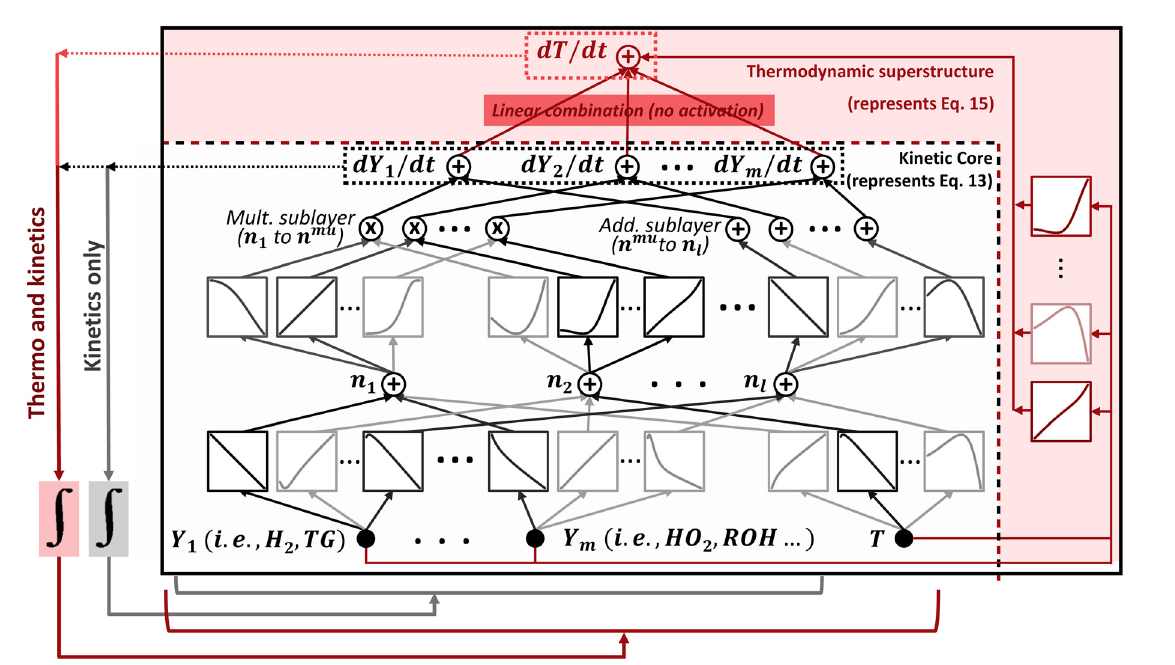
\includegraphics[width=0.95\textwidth]{ChemKAN_report_assets/chemkan_architecture_paper_fig2.png}
\caption{ChemKAN architecture proposed in Figure~2 of Koenig et al.~\cite{Koenig_2025}. The grey kinetic core maps the thermochemical state to species rates. The red thermodynamic superstructure combines these rates linearly and adds a correction KAN to obtain the temperature rate. The source article is published under CC BY-NC 4.0.}
\label{fig:chemkan_architecture}
\end{figure}

The two-stage training process changes which state is integrated, not Eqs.~(13)--(17). In Stage~1, only $\widetilde{\mathbf{u}}$ is integrated and temperature is supplied externally: it is constant for biodiesel and read from a dense observed/reference interpolant for hydrogen and methane. In Stage~2, the complete state $\mathbf{u}=[\widetilde{\mathbf{u}},T]$ is integrated and the kinetic and thermodynamic parameter groups are optimized together.

\paragraph{Loss.}
The printed ChemKAN objective is~\cite{Koenig_2025}
\begin{align}
\mathcal{L}(\boldsymbol{\theta})
&=\mathcal{L}_{\mathrm{MSE}}(\boldsymbol{\theta})
 +\mathcal{L}_{\mathrm{PINN}}(\boldsymbol{\theta}) \notag\\
&=\frac{1}{n^*}\sum_{j=1}^{N_t}\sum_{k=1}^{n^*}
\left(\widehat{u}^{\mathrm{pred}}_k(t_j,\boldsymbol{\theta})
      -\widehat{u}^{\mathrm{obs}}_k(t_j)\right)^2 \notag\\
&\quad+\alpha_{\mathrm{PINN}}
\sum_{i=1}^{N_e}\sum_{j=1}^{N_t}
\left|\sum_{k=1}^{m}
\frac{N_i^kW_i\left(Y^{\mathrm{pred}}_{k,j}-Y^{\mathrm{pred}}_{k,1}\right)}{W_k}\right|,
\end{align}
where
\begin{equation}
 n^*=\begin{cases}
 m,&\text{Stage 1},\\
 m+1,&\text{Stage 2}.
 \end{cases}
\end{equation}
The conservation term is evaluated at every time point for every conserved element and weighted by $\alpha_{\mathrm{PINN}}=10^{-4}$. The paper uses only the MSE term for biodiesel, while hydrogen uses the MSE plus the element-conservation term~\cite{Koenig_2025}. The methane extension follows the hydrogen-style loss. The printed MSE averages over modeled states but sums over time. For reporting, this project also uses
\begin{equation}
    \mathrm{MSE}_{\mathrm{time\text{-}avg}}=\frac{\mathcal{L}_{\mathrm{MSE}}}{N_t},
\end{equation}


The released Julia biodiesel example instead
uses \texttt{Flux.mse}, which averages over
both state variables and observation times.
The time-averaged convention is therefore
used for numerical comparisons in this report,
while the original training objective is
retained where required for reproduction.
Each figure and table identifies the
loss convention used for its results.

\subsection{Data generation and preparation}

\subsubsection{Biodiesel production}

The biodiesel benchmark is an isothermal six-species kinetic system. The paper uses activation energies $E_a=[14.54,6.47,14.42]$~kcal~mol$^{-1}$ and $\ln A=[18.60,7.93,19.13]$ for reactions 1--3, respectively~\cite{Koenig_2025}. Temperatures are randomly sampled from 323--343~K, initial TG and ROH concentrations are sampled uniformly from 0.5--2, all other species start at zero, and 20 training plus 10 test trajectories are generated over 30~s with 30 sampled times~\cite{Koenig_2025}.

A source-level discrepancy exists between the printed reaction ordering and the released biodiesel example. The released code uses $E_a [\cdot, \mathbf{14.42}, \mathbf{6.47}]$~kcal~mol$^{-1}$ and $\ln A=[\cdot,\mathbf{19.13},\mathbf{7.93}]$. Controlled datasets and training runs were produced for both orderings. The released-code ordering more closely reproduces the species levels shown in the paper's Figure 3: DG reaches about 0.47 and MG about 0.17, consistent with the figure's 0–0.6 and 0–0.2 axes, whereas the paper-text ordering gives about 0.29 and 0.325, so the MG curve would exceed its axis. The main author-matched biodiesel reproduction therefore uses the released-code ordering and keeps the paper-order experiment separate~\cite{ChemKANRepo2026}.

The paper's Figure~3 and Figure~6 unseen condition is
\begin{equation}
[\mathrm{TG}]_0=1.94,\quad[\mathrm{ROH}]_0=1.43,\quad
[\mathrm{DG}]_0=[\mathrm{MG}]_0=[\mathrm{GL}]_0=[\mathrm{R'CO_2R}]_0=0,\quad T=334.8~\mathrm{K}.
\end{equation}

The main biodiesel figure runs use \texttt{biodiesel\_v2.npz}, which was
generated in Python from the released-code kinetics and the authors' initial
conditions using SciPy LSODA with \(\texttt{rtol}=10^{-10}\) and
\(\texttt{atol}=10^{-12}\). These trajectories are used as the training
targets. PyTorch ChemKAN training uses \texttt{torchdiffeq}'s Tsit5 solver
with \(\texttt{rtol}=10^{-2}\) and \(\texttt{atol}=10^{-6}\). For the
biodiesel figure pipeline, the final-checkpoint losses used in Figures~4
and~5A and the trajectories used in Figures~3 and~6 are re-evaluated in
double precision with Tsit5 at \(\texttt{rtol}=10^{-10}\) and
\(\texttt{atol}=10^{-12}\), so that the reported model error is not dominated
by the deliberately loose training solve. The per-epoch histories in
Figure~5B retain the training-solver evaluations.

A separate implementation-comparison experiment uses training arrays exported
from the released Julia example. For that dataset, an independent Python
reconstruction using SciPy's LSODA solver
~\cite{virtanen2020scipy}
with \(\texttt{rtol}=10^{-12}\) and
\(\texttt{atol}=10^{-14}\) serves only as a cross-check and is not used as a
training target. The released Julia example uses
\texttt{AutoTsit5(Rosenbrock23)} for both reference-data
generation and ChemKAN integration. Reference trajectories
are generated from the known Arrhenius reaction equations
using the OrdinaryDiffEq default tolerances
($\mathrm{reltol}=10^{-3}$, $\mathrm{abstol}=10^{-6}$).
During training, ChemKAN-predicted derivatives are integrated
with $\mathrm{reltol}=10^{-2}$ and $\mathrm{abstol}=10^{-6}$,
and the resulting trajectories are compared against the
reference data. The same settings are used for validation
and plotting, without a separate evaluation tolerance.

\subsubsection{Hydrogen--air combustion}

The hydrogen data were generated with Cantera~\cite{cantera} using \texttt{h2o2.yaml}. Argon was omitted, leaving nine tracked species mass fractions plus temperature. The Cantera reactor integrations use \(\texttt{rtol}=10^{-9}\) and \(\texttt{atol}=10^{-15}\). The design contains 36 combinations of
$
T_0\in\{950,1000,1050,1100,1150,1200\}\ \mathrm{K}
$
and
$
\phi\in\{0.5,0.7,0.9,1.1,1.3,1.5\};
$
35 are used for training, while \((T_0=1150\,\mathrm{K},\phi=1.3)\) is held out. The printed paper omits \(\phi=0.5\) from its list despite stating that 36 combinations were used; the authors later clarified that \(0.5\) belongs to the grid~\cite{Koenig_2025,ChemKANAuthors2026}. The local training dataset contains 100 uniformly spaced output times over the \(0.6\)-ms trajectory, and a separately generated 20,000-point Cantera temperature cache supplies the linear temperature interpolant used during Stage~1. The authors clarified that their original trajectories were instead generated with Arrhenius.jl using CVODE\_BDF and checked against Cantera; direct Cantera generation is therefore a choice of this reproduction rather than a claim about the authors' original pipeline~\cite{ChemKANAuthors2026}.

The final author-matched architecture has hidden width \(3\), five RBF basis functions per edge, \(n_{\mathrm{mu}}=3\), no base activation, and 344 trainable parameters. Both training stages use Adam with learning rate \(2\times10^{-3}\) and Tsit5 with \(\texttt{rtol}=10^{-6}\) and \(\texttt{atol}=10^{-8}\). 
The PyTorch implementation integrates
min--max-normalized states while the ODE solver
advances physical time $t$ in seconds.
A reference time scale $t_{\mathrm{ref}}$ is
used to scale the complete raw ChemKAN
right-hand side:


\[
\frac{d\hat{\mathbf{u}}}{dt}
=
\frac{
F(\hat{\mathbf{u}},\boldsymbol{\theta})
}{
t_{\mathrm{ref}}
}
\]

This scaling is analogous to the released biodiesel example, which divides its
learned right-hand side by a constant factor of \(50\), although its trajectory
spans only \(30\,\mathrm{s}\). For hydrogen, we instead choose the full
\(0.6\)-ms trajectory horizon as \(t_{\mathrm{ref}}\). Because no hydrogen
source code was released, both this scaling and the value of
\(t_{\mathrm{ref}}\) are reported as PyTorch-reproduction choices rather than
as author-specified settings.

\subsubsection{Methane-air oxidation extension}

Methane is not part of the original ChemKAN paper and is treated as a transfer experiment rather than a reproduction target. The extension uses the GRI-Mech~3.0
chemical mechanism~\cite{GRIMech30}. Argon is omitted because it remains a constant-zero inert species in the selected setup, leaving 52 species plus temperature and a 1,892-parameter ChemKAN. The initial-condition grid mirrors the hydrogen design: $T_0\in\{1400,1450,1500,1550,1600,1650\}$~K and $\phi\in\{0.5,0.7,0.9,1.1,1.3,1.5\}$, with $(T_0=1550\,\mathrm{K},\phi=1.3)$ held out. Each trajectory contains 100 observation times over 5~ms, and a 20,000-point temperature cache is used in Stage~1. Reference trajectories were generated with Cantera using an adiabatic constant-pressure reactor at an initial pressure of 1~atm.

The model uses the same author-matched architecture pattern and loss as hydrogen. The normalized trajectory coordinate uses $t_{\mathrm{ref}}=5$~ms $=5\times10^{-3}$~s, equal to the full methane trajectory horizon, with the normalized right-hand side divided by $t_{\mathrm{ref}}$ while the solver advances physical time in seconds. This follows the same PyTorch normalized-time formulation as the hydrogen reproduction.


The methane experiment followed the same two-stage
training formulation as hydrogen. 
Stage~1 continued to approximately
54,800 epochs, and its archived
epoch-50,000 checkpoint was used
to initialize Stage~2, which was
trained for 200,000 epochs. Training used Adam
with learning rate $2\times10^{-3}$, the Tsit5
solver with $\mathrm{rtol}=10^{-6}$ and
$\mathrm{atol}=10^{-8}$, float32 precision,
and direct automatic differentiation. The complete Stage-2 training history and
checkpoints were preserved. Because optimization
remained non-monotonic, archived checkpoints
were independently evaluated over complete
trajectories from the initial conditions.
The primary evaluation model was selected using
the mean time-averaged MSE across the 35 training
conditions, without using the held-out condition
for checkpoint selection. The selected checkpoint corresponds to Stage-2 epoch 180,000 because epoch 200,000 coincided with a spike. The final epoch-200,000
checkpoint was retained and evaluated separately.

\subsection{Experiment design and reproducibility controls}

The following controls were used throughout the project:
\begin{itemize}
    \item Predefined reproduction targets were mapped to the original paper's figures and table (biodiesel Figures~3--6; hydrogen Figures~7--8 and Table~I).
    \item Legacy experiments were preserved instead of overwritten. Author-clarified experiments use separate directories and explicit provenance, preventing post-hoc relabeling.
    \item Every major run stores its configuration, training history, checkpoint(s), run log, data-file hash, and, for key checkpoints, SHA-256 hashes.
    \item Random seeds are fixed for controlled comparisons. Single-seed findings are reported as single-run evidence rather than population-level claims.
    \item Train/test preprocessing is documented explicitly. Where released code uses a different convention from the paper, both conventions are recorded rather than silently reconciled.
    \item Evaluation code is separated from training: saved checkpoints are re-evaluated on fixed reference datasets and common diagnostic grids.
    \item Numerical sensitivity backends are validated independently before being used in long training runs.
\end{itemize}

The implementation, experiment configurations, selected checkpoints, evaluation artifacts, and computational environment are documented in the accompanying ChemKAN release repository. The repository also preserves the pinned `torchdiffeq` source distribution, including its license and provenance information.

The main PyTorch reproduction uses the explicit Tsit5 integrator from `torchdiffeq` \cite{torchdiffeq}. It does not automatically switch to a stiff solver. This differs from the released Julia biodiesel example, which uses `AutoTsit5(Rosenbrock23)` and can switch from Tsit5 to Rosenbrock23 when stiffness is detected \cite{ChemKANRepo2026}. The printed ChemKAN paper states Tsit5 for the ChemKAN/FSA solve \cite{Koenig_2025}.



\subsection{Forward Sensitivity Analysis}

The proposal specified forward sensitivity analysis (FSA) for propagating parameter derivatives through the ODE solver. A continuous FSA backend was therefore implemented in addition to direct automatic differentiation. For an integrated state $\mathbf{x}(t)$,
\begin{equation}
    \frac{\dd\mathbf{x}}{\dd t}=F(\mathbf{x},t,\boldsymbol{\theta}),
\end{equation}
and parameter vector $\boldsymbol{\theta}$, define
\begin{equation}
    S(t)=\frac{\partial\mathbf{x}(t)}{\partial\boldsymbol{\theta}}.
\end{equation}
Differentiating the state equation with respect to $\boldsymbol{\theta}$ gives the standard forward-sensitivity system~\cite{SciMLSensitivityMath}
\begin{equation}
    \frac{\dd S}{\dd t}=J_xS+J_{\boldsymbol{\theta}},\qquad
    J_x=\frac{\partial F}{\partial\mathbf{x}},\qquad
    J_{\boldsymbol{\theta}}=\frac{\partial F}{\partial\boldsymbol{\theta}},\qquad
    S(t_0)=0.
\end{equation}
The initial sensitivity is zero because the reactor initial condition does not depend on the learnable network parameters.

The solver advances the physical state and the sensitivity matrix simultaneously. In compact notation,
\begin{equation}
    \mathbf{z}(t)=\big(\mathbf{x}(t),S(t)\big),
\end{equation}
with
\begin{equation}
    \frac{\dd\mathbf{z}}{\dd t}
    =\left(F(\mathbf{x},t,\boldsymbol{\theta}),\;J_xS+J_{\boldsymbol{\theta}}\right).
\end{equation}
Here $\dd\mathbf{z}/\dd t$ is only the time derivative of the augmented state. It is not a derivative of $\mathbf{z}$ with respect to $\mathbf{x}$. In code, the physical state and sensitivity matrix are combined into a single augmented tensor for ODE integration; mathematically, \(S\) remains the state-by-parameter sensitivity matrix.

In PyTorch, the existing \texttt{KineticDynamics}/\texttt{ChemKANDynamics} right-hand side is called through \texttt{torch.func.functional\_call}; the model dynamics are therefore not reimplemented for FSA. \texttt{torch.\allowbreak  func.jacrev} forms the state and parameter Jacobians, and \texttt{torch.func.vmap} applies the calculation independently over trajectories in a batch. The augmented system is integrated with the same run-level solver and tolerances. After integration, the parameter gradient is assembled as
\begin{equation}
    \frac{\dd L}{\dd\boldsymbol{\theta}}
    =\sum_j S(t_j)^{\mathsf T}\frac{\partial L}{\partial\mathbf{x}(t_j)}.
\end{equation}
For Stage~1, $\mathbf{x}=\widetilde{\mathbf{u}}$ and temperature is an external input. For Stage~2, $\mathbf{x}=\mathbf{u}$, so $J_x$ automatically carries species--temperature coupling into the sensitivity equations.

The FSA implementation integrates the physical state
and its parameter sensitivities as a single augmented
system. The adaptive Tsit5 solver applies the specified
relative and absolute tolerances to the entire augmented
state using its default error norm. In contrast,
direct differentiation integrates only the physical
state and differentiates the numerical solver computation.

Consequently, the two approaches may use different
adaptive integration steps even when their nominal
solver tolerances are identical. This distinction is
considered when comparing training behavior, but it
does not imply that either differentiation backend
is universally preferable.

\subsection{Evaluation metrics and baselines}

The proposal defined training/test MSE, generalization to held-out initial conditions, noise-free test error under noisy training, and inference time as the primary metrics. The report retains those metrics and adds combustion-specific diagnostics where a single aggregate MSE can hide physically important behavior.

\begin{table}[H]
\centering
\small
\caption{Primary evaluation metrics.}
\label{tab:metrics}
\begin{tabularx}{\textwidth}{@{}p{0.25\textwidth}X@{}}
\toprule
\textbf{Metric} & \textbf{Purpose} \\
\midrule
Trajectory MSE & Primary normalized prediction error. The printed Eq.~(18) averages over state variables and sums over time. For cross-plot reporting, $\mathrm{MSE}_{\mathrm{time\text{-}avg}}=\mathcal{L}_{\mathrm{MSE}}/N_t$ is also reported. The released biodiesel Julia example uses this time-averaged form through \texttt{Flux.mse}; hydrogen training retains Eq.~(18). \\
Generalization & Held-out initial-condition error; for hydrogen, a reconstructed $21\times21$ grid (441 conditions) is also evaluated. \\
Noise robustness & Clean-ground-truth test MSE after training on noisy observations; train-loss increase is compared with the irreducible noise floor. \\
Ignition behavior & Temperature rise, ignition delay defined as $\operatorname*{arg\,max}_t \dd T/\dd t$, and integration failures. \\
Complexity & Trainable parameter count and model organization. \\
Efficiency & End-to-end trajectory integration runtime under a common task definition; speed-up is traditional-solver runtime divided by ChemKAN runtime. \\
\bottomrule
\end{tabularx}
\end{table}


For combustion, ignition delay is defined
as the time of maximum temperature-rise rate,
following the original ChemKAN study:
\begin{equation}
t_{\mathrm{ign}}
=
\operatorname*{arg\,max}_{t}
\frac{\mathrm{d}T}{\mathrm{d}t}.
\end{equation}
Numerically, the temperature derivative is
estimated on the diagnostic time grid using
finite differences. For initial condition $i$,
the absolute relative ignition-delay error is
\begin{equation}
e_{\mathrm{ign}}^{(i)}
=
\frac{
\left|
t_{\mathrm{ign,pred}}^{(i)}
-
t_{\mathrm{ign,ref}}^{(i)}
\right|
}{
t_{\mathrm{ign,ref}}^{(i)}
}.
\end{equation}
The reported median absolute relative error
is $100\%$ times the median of
$e_{\mathrm{ign}}^{(i)}$ across the evaluated
conditions. For the hydrogen Figure~8B
comparison, this comprises 30 initial
conditions.


DeepONet is reimplemented for the biodiesel
architectural comparison. For combustion,
ChemNODE is used as a literature baseline,
with its reported results taken from the
original ChemNODE study~\cite{OWOYELE2022100118}
rather than from an independent reimplementation.
These published results provide context for the
comparison but are not treated as direct
same-hardware measurements. Traditional numerical
references are Cantera for combustion and direct
integration of the known biodiesel kinetics.

Cantera has two distinct roles in the combustion experiments. First, it generates the detailed-chemistry reference trajectories against which ChemKAN accuracy is measured. Thus, Cantera is not a competing predictor in the accuracy metric; ChemKAN error is measured relative to the Cantera solution. Second, computational efficiency is evaluated separately by re-running the \emph{same initial-value problem} with Cantera and the trained ChemKAN model on identical hardware, with model/mechanism loading outside the timed region. The speed-up is defined as
\begin{equation}
    S_{\mathrm{speed}} = \frac{t_{\mathrm{traditional}}}{t_{\mathrm{ChemKAN}}}.
\end{equation}
A value greater than one indicates acceleration. Accuracy and runtime are reported together, because a faster surrogate is only useful if the loss of fidelity is acceptable.

\section{Results and Evaluation}

\subsection{Biodiesel reproduction}

The initial biodiesel reproduction was based on the paper alone and required a substantial series of ablations. Several qualitative dynamics could be learned, but the published loss levels and robustness trends were not reproduced consistently. One early assumption was multiplicative observation noise. The author clarification later specified additive Gaussian noise of the form $\mathcal{N}(0,1)$ times each species maximum and the requested noise percentage, clipped at zero; the clarified dataset and final reproduction use this additive construction~\cite{ChemKANAuthors2026}. The released Julia example further established the no-base 156-parameter ChemKAN and exposed implementation details that differ from the printed paper~\cite{ChemKANRepo2026}.

A controlled reaction-order experiment used the same initial conditions, training settings, and seed while changing only the reaction-2/reaction-3 Arrhenius ordering. Aggregate losses were of similar scale, but the released-code ground truth produced DG and MG levels that match the y-axis ranges and trajectories of the published Figure~3 more closely. Because the authors did not explicitly confirm which ordering generated the published figure, this is reported as evidence rather than as a correction of the paper.

The strongest quantitative reproduction is the noise-floor behavior. Under the authors' released-example time-averaged loss, the 0$\rightarrow$1\% and 0$\rightarrow$5\% training-loss increments are close to the values stated in the paper, and the 15\% clean-test degradation is close to the reported approximately two-fold increase. Neural-scaling exponents are less stable across the reconstructed model-size set and the single training seed.

\begin{table}[htbp]
\centering
\small
\caption{Biodiesel reproduction results compared with the original ChemKAN study. MSE values follow the time-averaged convention.}
\label{tab:biodiesel_summary}
\begin{tabularx}{\textwidth}{@{}Xcc@{}}
\toprule
\textbf{Quantity} &
\textbf{Original study} &
\textbf{PyTorch reproduction} \\
\midrule
ChemKAN neural-scaling exponent (train/test)
& 1.0 / 0.6 & 1.49 / 0.372 \\
78-parameter ChemKAN error (train/test)
& $\sim10^{-4}$
& $4.79\times10^{-4}$ / $7.68\times10^{-4}$ \\
Training-loss increase, 0--1\% noise
& $3.78\times10^{-5}$ & $4.19\times10^{-5}$ \\
Training-loss increase, 0--5\% noise
& $9.64\times10^{-4}$ & $1.05\times10^{-3}$ \\
ChemKAN Clean-test error ratio, 15\% / 0\%
& $\sim2.0$ & $1.84$ \\
15\% clean-test error ratio,
DeepONet / ChemKAN
& $4.4$ & $2.73$ \\
\bottomrule
\end{tabularx}
\end{table}

\begin{figure}[htbp]
\centering
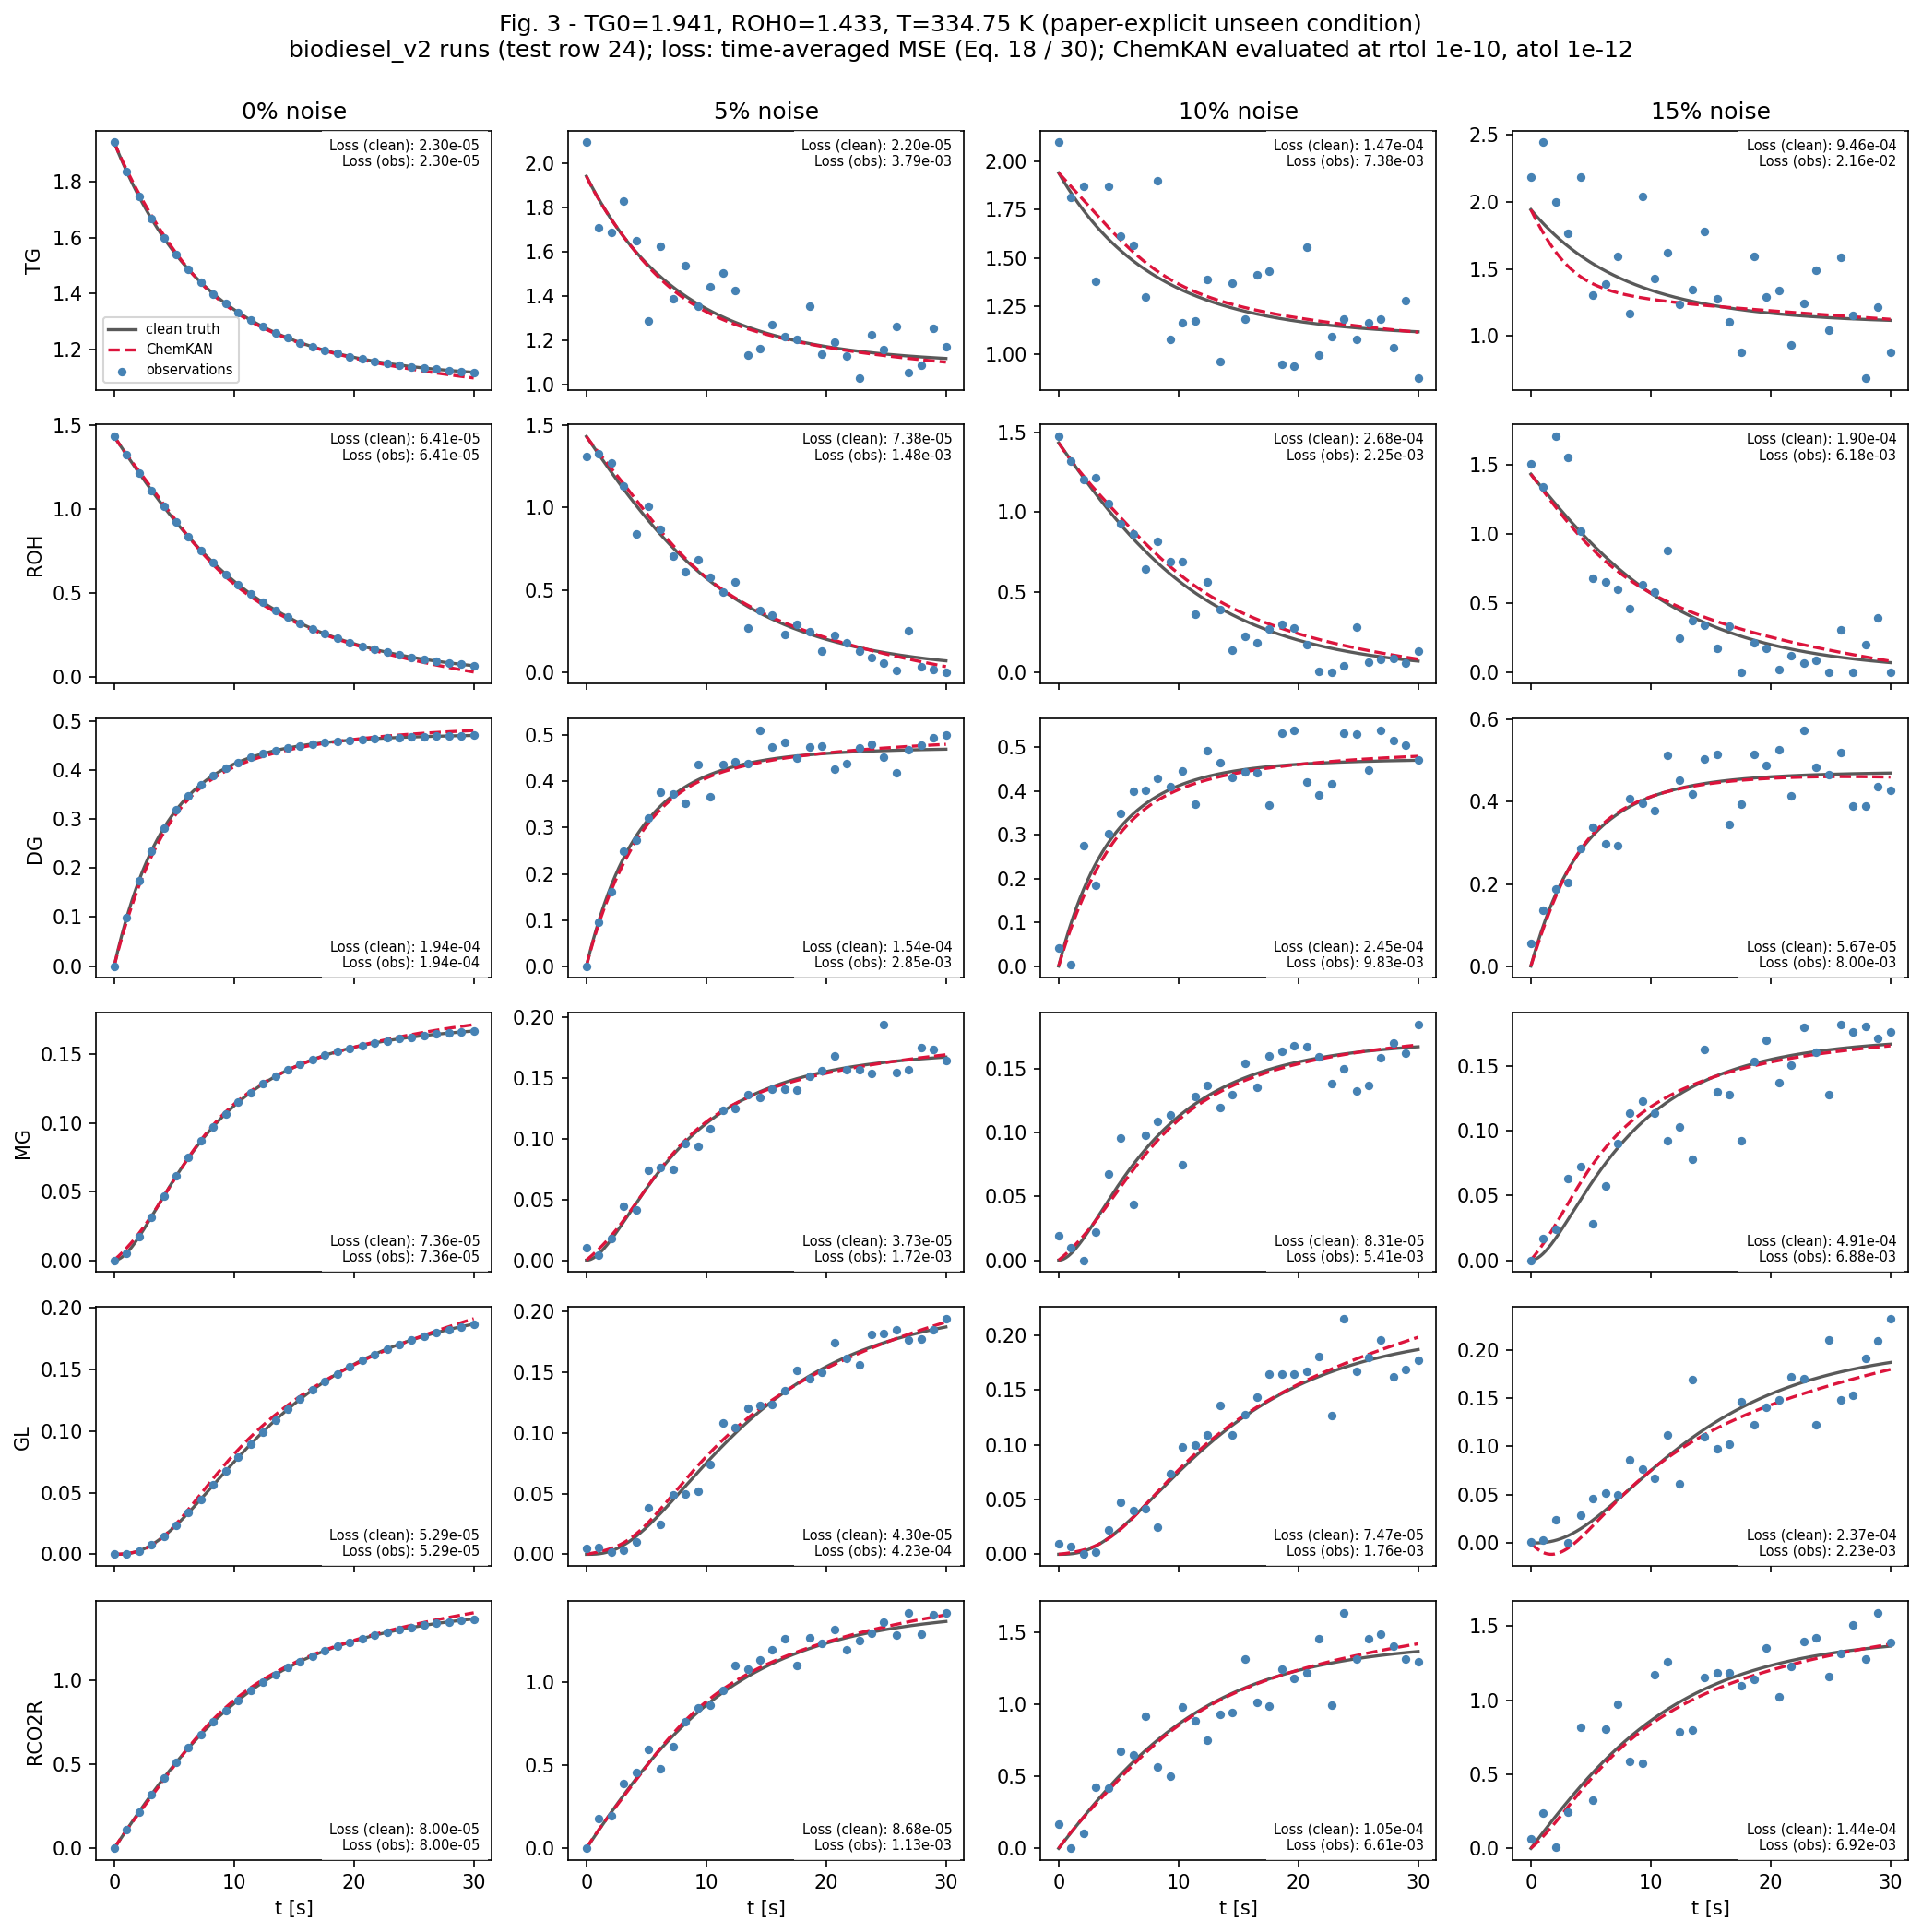
\includegraphics[width=0.97\textwidth]{ChemKAN_report_assets/biodiesel_fig03.png}
\caption{ChemKAN reproduction of the paper's Figure~3 unseen condition under 0\%, 5\%, 10\%, and 15\% observation noise. The initial condition is $[\mathrm{TG}]_0=1.94$, $[\mathrm{ROH}]_0=1.43$, all four other species initially zero, and $T=334.8$~K. The model was trained with Tsit5 at \texttt{rtol}$=10^{-2}$ and \texttt{atol}$=10^{-6}$; the displayed curves were re-evaluated at \texttt{rtol}$=10^{-10}$ and \texttt{atol}$=10^{-12}$. Each species uses its own y-axis scale, following the paper's presentation.}
\label{fig:biodiesel_trajectories}
\end{figure}

The DeepONet architecture was reconstructed using the
parameter count reported in the ChemKAN paper and the
branch-input dimensions clarified by the authors.
However, the exact activation functions, learning rate,
and time-input preprocessing were not fully specified. An initial ReLU-based implementation did not reproduce
the reported predictive behavior satisfactorily.
Consequently, additional controlled ablations were
conducted to investigate activation functions and
optimization settings. The selected reconstruction uses
tanh activations, raw physical time as the trunk input,
and an Adam learning rate of $10^{-2}$. This configuration is reported as the selected
behavior-matching reconstruction rather than an
exactly recovered author implementation.
The original ReLU experiments are retained as
diagnostic evidence.



\begin{figure}[htbp]
\centering
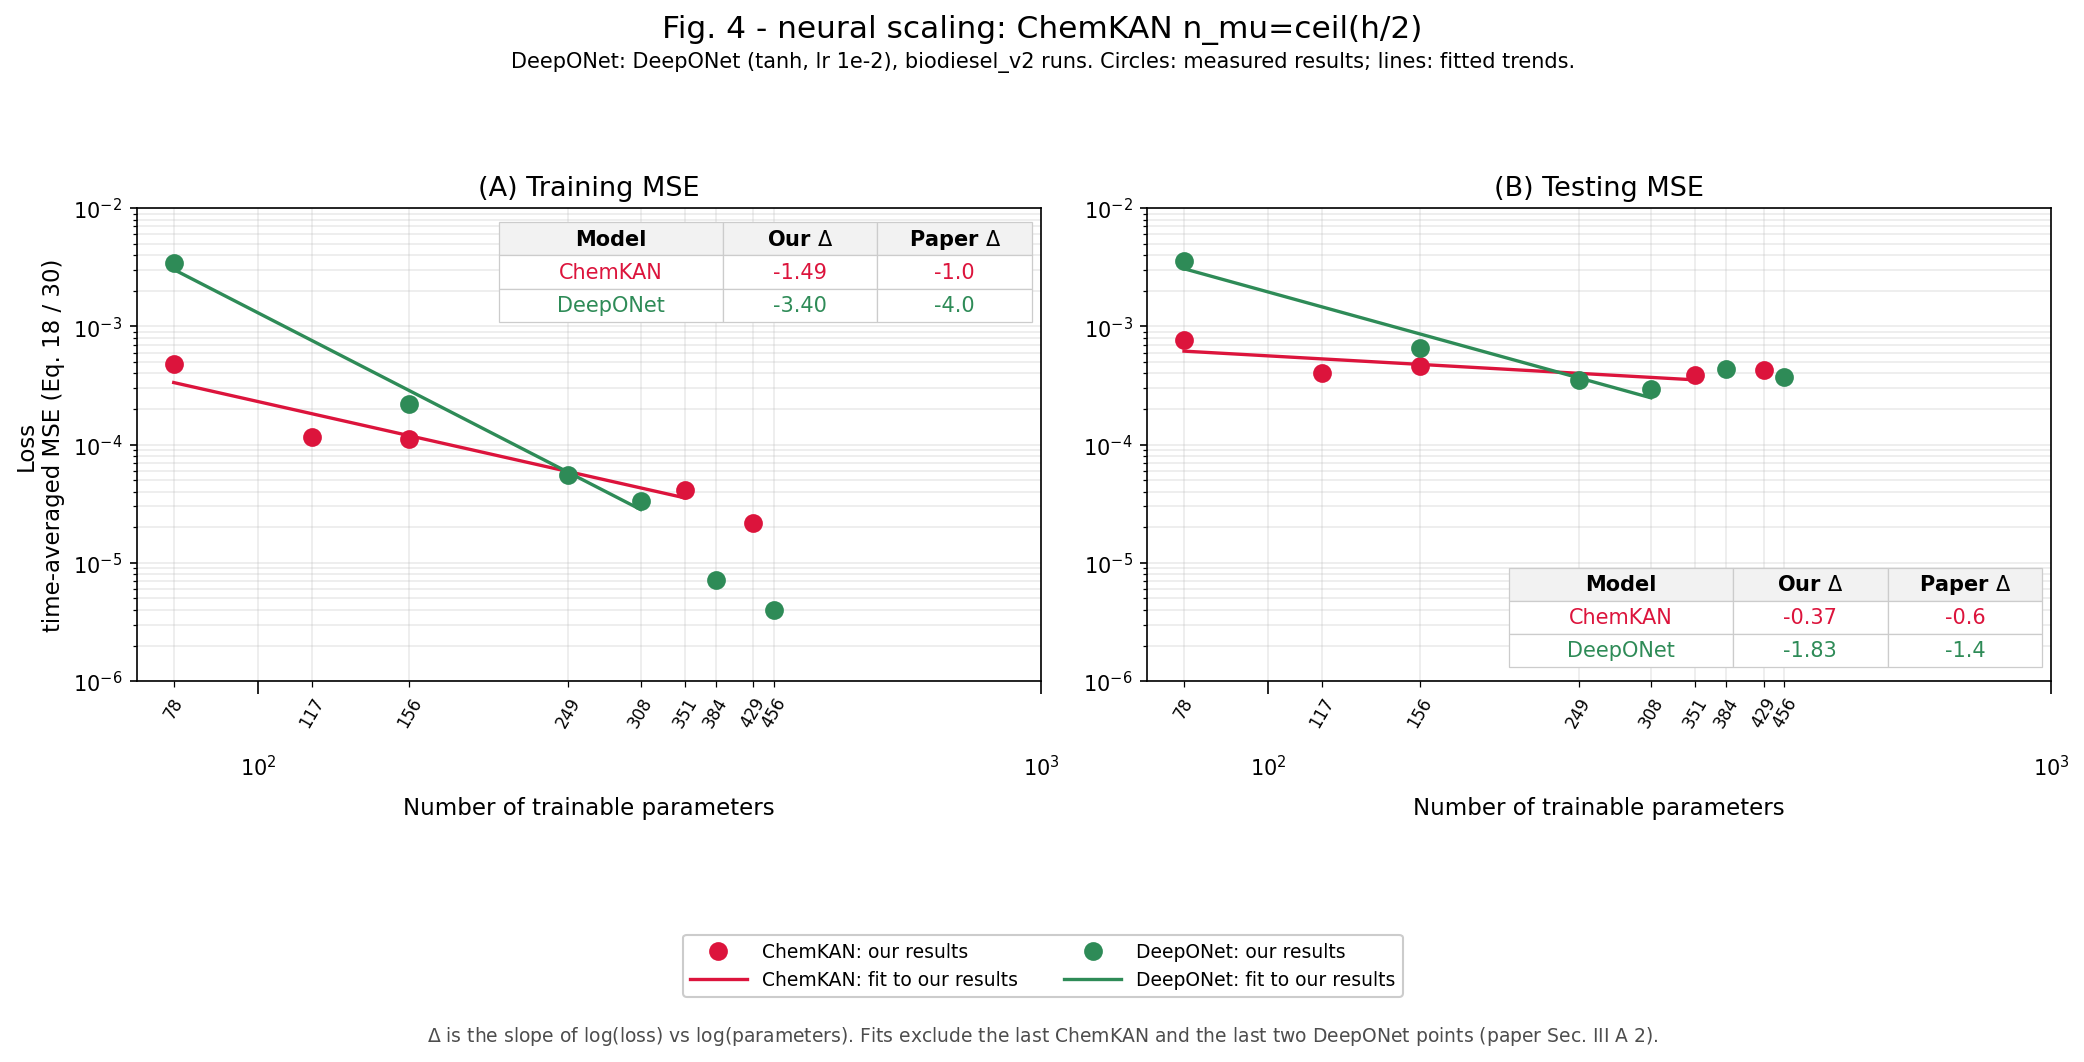
\includegraphics[width=0.85\textwidth]
{ChemKAN_report_assets/fig04_scaling.png}
\caption{Neural scaling on noise-free biodiesel data
(seed 0). Final-checkpoint time-averaged normalized
training and testing MSE are shown for ChemKAN
models trained for 5,000 epochs and the selected
tanh DeepONet reconstruction trained for 50,000
epochs. Log--log fits exclude the 429-parameter
ChemKAN and the 384- and 456-parameter DeepONets,
following the saturation exclusions described in
the original study. ChemKAN predictions are evaluated
with $\mathrm{rtol}=10^{-10}$ and
$\mathrm{atol}=10^{-12}$.}
\label{fig:biodiesel_scaling}
\end{figure}

\begin{figure}[htbp]
\centering
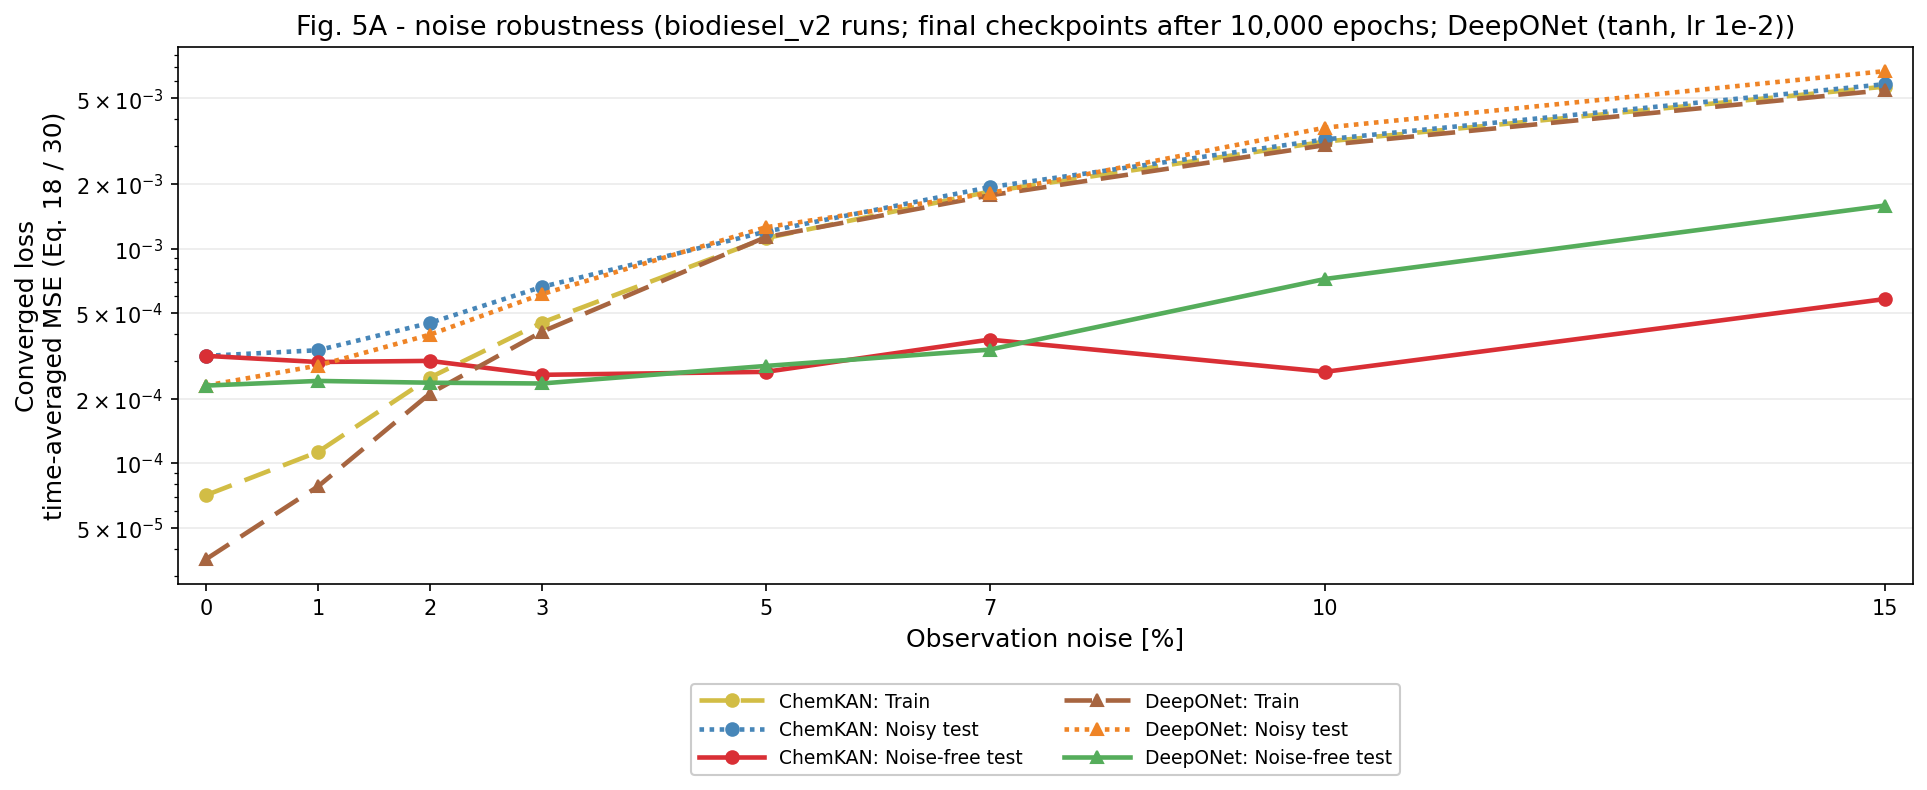
\includegraphics[width=0.85\textwidth]
{ChemKAN_report_assets/fig05a_noise.png}
\caption{Noise robustness of the 156-parameter
ChemKAN and 308-parameter tanh DeepONet after
10,000 training epochs (seed 0). The curves show
time-averaged normalized MSE against noisy training
observations, noisy held-out observations, and clean
held-out reference trajectories. The evaluation
uses the noise-level-specific normalization recorded
in the experiments. ChemKAN predictions are
evaluated with $\mathrm{rtol}=10^{-10}$ and
$\mathrm{atol}=10^{-12}$.}
\label{fig:biodiesel_noise}
\end{figure}


Figure~\ref{fig:biodiesel_noise} compares
the final checkpoints of the 156-parameter
ChemKAN and the selected 308-parameter tanh
DeepONet reconstruction, each trained for
10,000 epochs with seed 0 at the corresponding
observation-noise level. The DeepONet uses
raw physical time as its trunk input and
an Adam learning rate of $10^{-2}$.

At lower noise levels, the selected DeepONet
achieved comparable or lower clean-test MSE
in several cases. At 10\% and 15\% noise,
ChemKAN achieved approximately 2.7-fold
lower clean-test MSE. The 15\% ratio was
2.73, compared with 4.4 reported in the
original study. These single-seed results
support a ChemKAN advantage at higher noise
levels, but not uniform superiority
across all tested noise levels.


\begin{figure}[htbp]
\centering
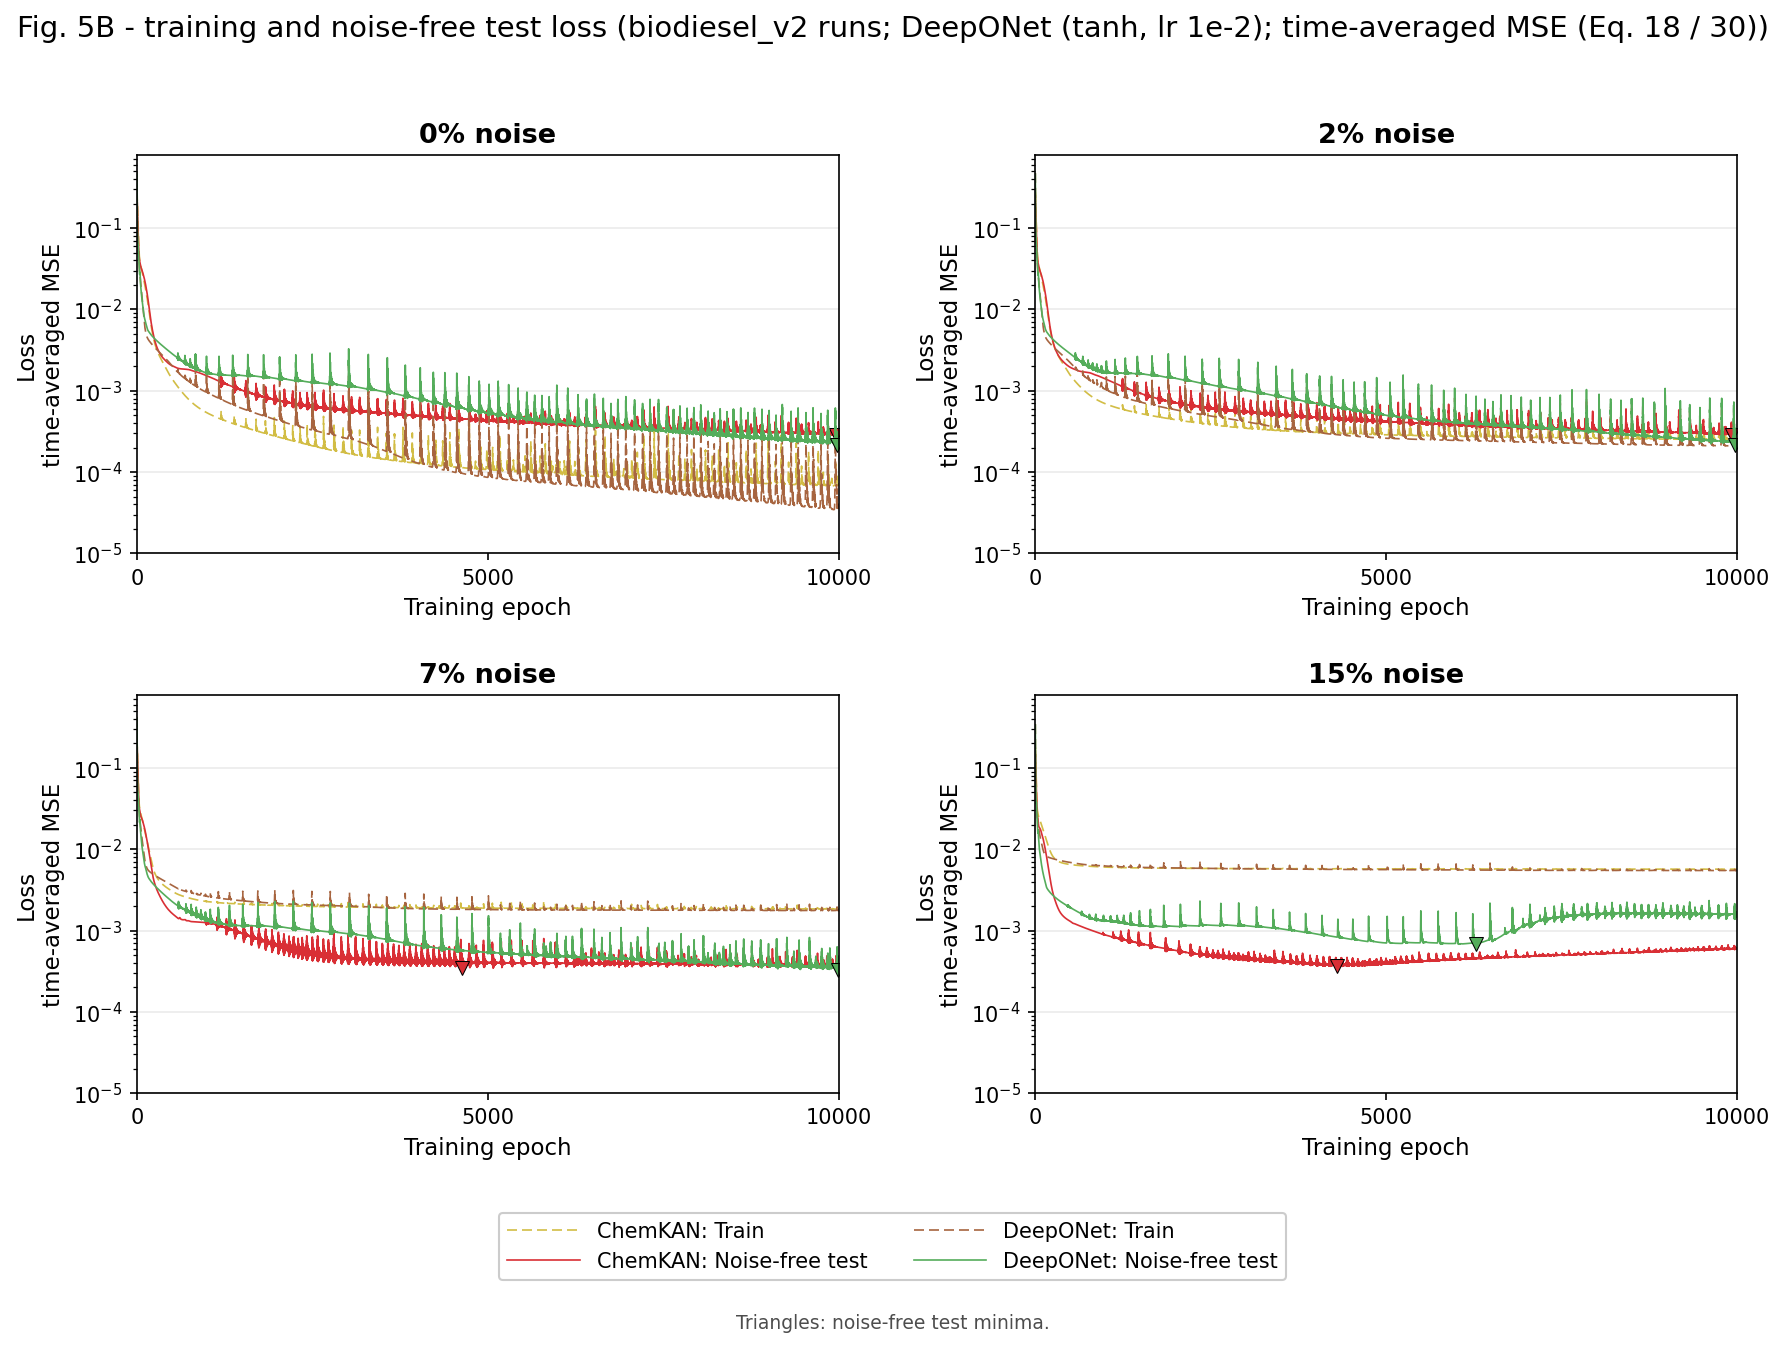
\includegraphics[width=0.85\textwidth]
{ChemKAN_report_assets/fig05b_loss_histories.png}
\caption{Recorded training and clean-test MSE
histories of ChemKAN and the selected tanh DeepONet
at 0\%, 2\%, 7\%, and 15\% observation noise.
MSE is averaged over species and observation times.
The ChemKAN histories use the training-solver
tolerances $\mathrm{rtol}=10^{-2}$ and
$\mathrm{atol}=10^{-6}$. Triangles indicate the
minimum recorded clean-test MSE.}
\label{fig:biodiesel_histories}
\end{figure}

\begin{figure}[htbp]
\centering
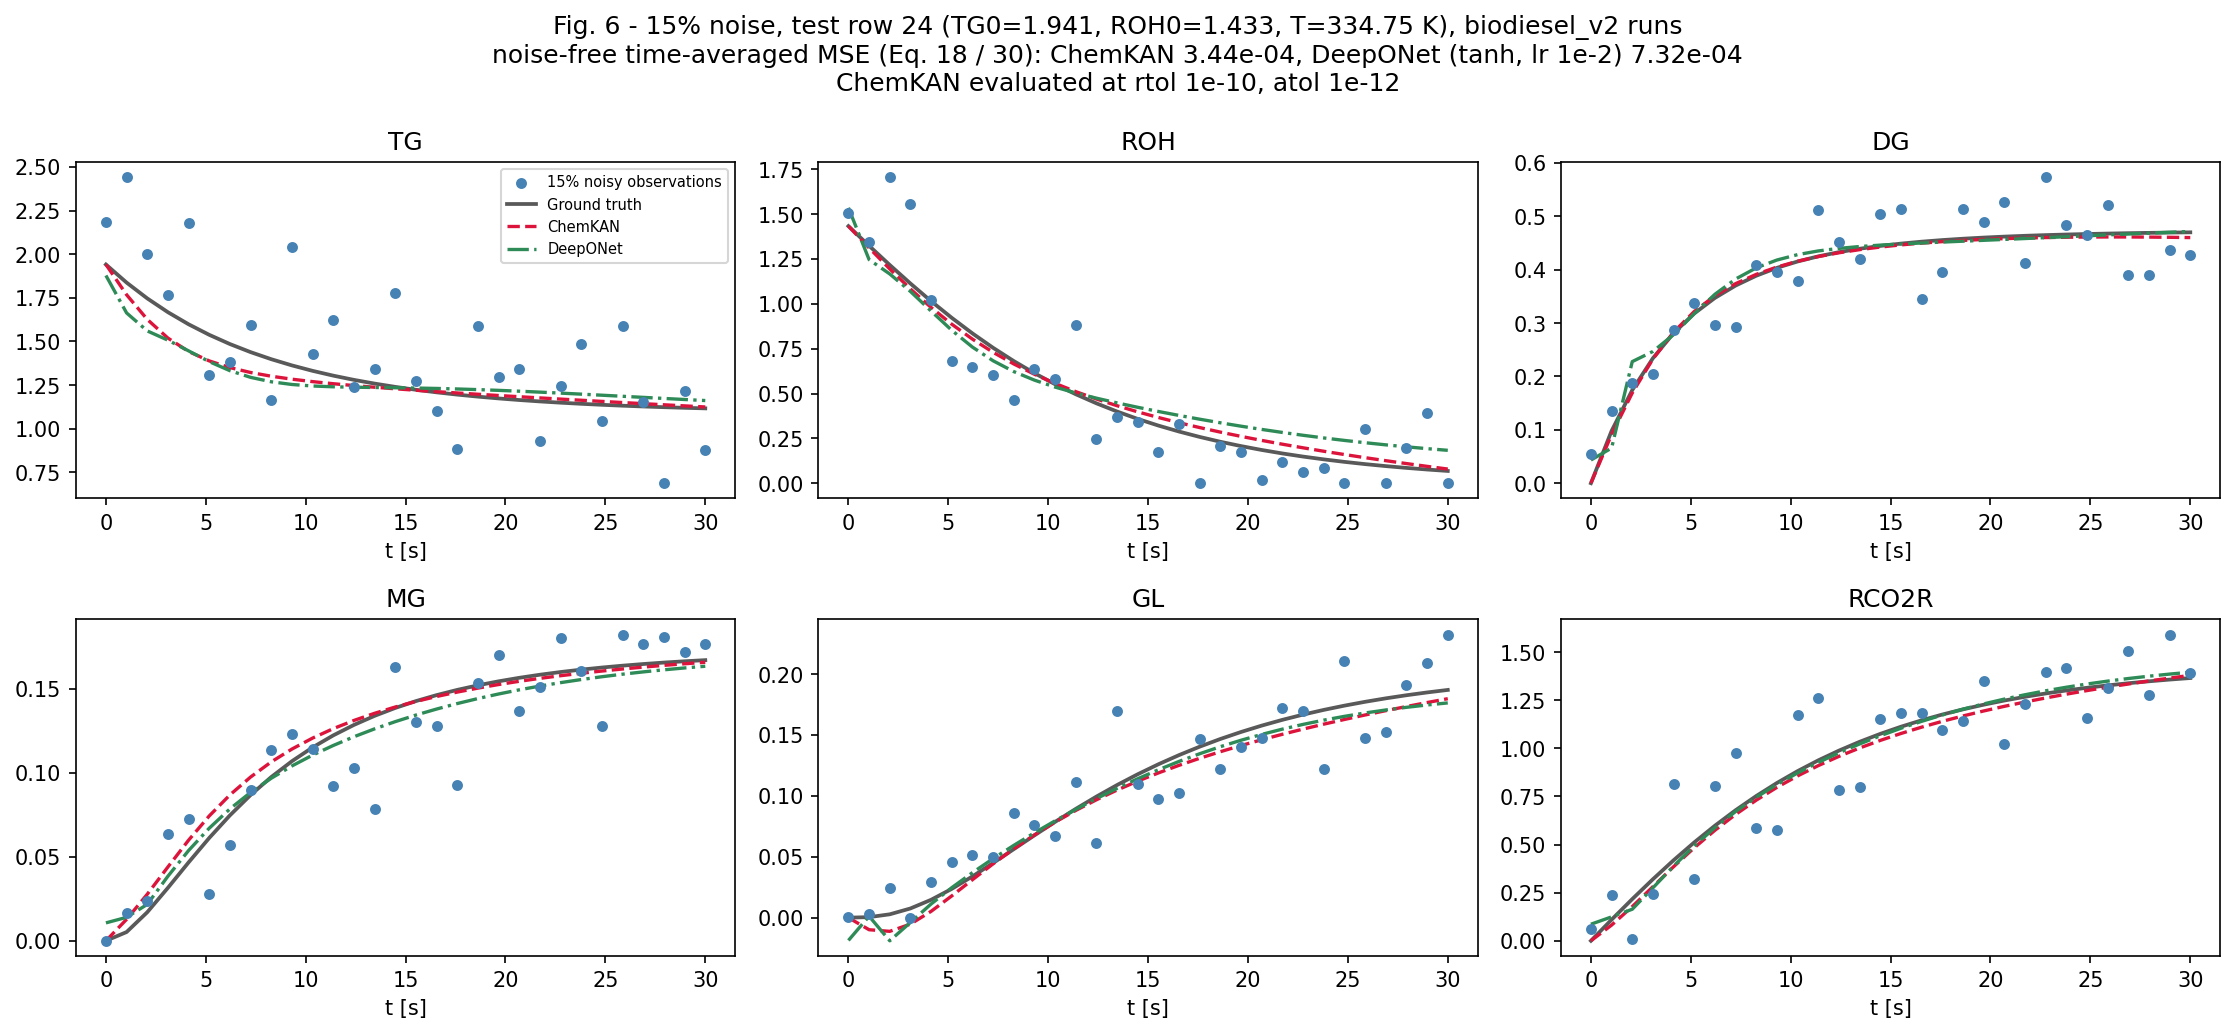
\includegraphics[width=0.9\textwidth]
{ChemKAN_report_assets/fig06_profiles_15pct.png}
\caption{Biodiesel species trajectories for the
unseen initial condition
$[\mathrm{TG}]_0=1.940826$,
$[\mathrm{ROH}]_0=1.433298$, and
$T=334.7486$~K, using ChemKAN and DeepONet models
trained with 15\% observation noise. The curves
correspond to the final 156-parameter ChemKAN and
308-parameter tanh DeepONet checkpoints.
Time-averaged clean-test MSE for this trajectory
is $3.4408\times10^{-4}$ for ChemKAN and
$7.3175\times10^{-4}$ for DeepONet.}
\label{fig:biodiesel_profiles}
\end{figure}


\subsection{Hydrogen-air combustion reproduction}

Hydrogen was the most difficult reproduction target. Under the initial paper-only protocol, the species trajectories could be learned to a useful qualitative level, but the Stage-2 temperature dynamics often failed to ignite and the loss remained high. Diagnostics showed that the thermodynamic linear layer initially produced a temperature derivative with insufficient magnitude. The author clarification supplied several missing settings, including no base activation, five RBF basis functions, min--max-normalized inputs, thermodynamic linear weights initialized to $10^{-5}$, a 100-point training grid, a separate dense temperature interpolant, and a $10^5$--$2\times10^5$ epoch range per stage~\cite{ChemKANAuthors2026}.

The normalized-state formulation also changes the scale of the ODE right-hand side: dividing the complete normalized RHS by the 0.6~ms trajectory horizon increases its physical-time magnitude by $1/t_{\mathrm{ref}}$. Together with the clarified architecture and initialization, this removed the earlier temperature-rate magnitude mismatch and allowed the model to learn ignition. The individual causal contribution of the time scaling versus the other clarified changes was not isolated in a single-factor ablation, so the report does not attribute the recovery to one change alone.


The main hydrogen reproduction used 100,000 Stage-1
epochs followed by 200,000 Stage-2 epochs.
Stage~1 exhibited non-monotonic optimization
behavior, with its lowest logged time-averaged MSE
of $5.334\times10^{-4}$ at epoch 60,037.
The fixed 100k checkpoint was retained as the
starting point for Stage~2. In Stage~2, the lowest logged time-averaged MSE
was $4.548\times10^{-4}$ at epoch 199,954,
while the epoch-200,000 value was
$6.360\times10^{-4}$. Logged training errors are
distinguished from the independent evaluations
of the saved checkpoints.


\begin{table}[htbp]
\centering
\small
\caption{Hydrogen Stage-2 training progression
and independent checkpoint evaluation.
Logged training MSE is recorded at the specified
epoch, while held-out MSE is obtained by evaluating
the corresponding checkpoint. Both use
time-averaged normalized MSE over 100 time points. Ignition-delay error denotes the median
absolute relative error over the 30
Figure~8B initial conditions.
}
\label{tab:hydrogen_checkpoints}
\begin{tabular}{@{}rrrr@{}}
\toprule
\textbf{Epoch} &
\textbf{Train MSE} &
\textbf{Held-out MSE} &
\textbf{Ignition-delay error} \\
\midrule
100k & $1.388\times10^{-3}$ &
       $8.170\times10^{-4}$ & 3.69\% \\
150k & $7.425\times10^{-4}$ &
       $4.526\times10^{-4}$ & 1.64\% \\
200k & $6.360\times10^{-4}$ &
       $3.507\times10^{-4}$ & 1.36\% \\
\bottomrule
\end{tabular}
\end{table}


The epoch-200,000 checkpoint was used for
the main hydrogen evaluation as the endpoint
of the planned Stage-2 training budget,
consistent with the authors' reported
training range. Its held-out MSE and
ignition-delay error are reported alongside
those of the earlier archived checkpoints
to illustrate training progression.

A reconstructed $21\times21$ grid (441 conditions) was evaluated in float64 with Tsit5 at \texttt{rtol}$=10^{-10}$ and \texttt{atol}$=10^{-12}$. The time-averaged normalized trajectory MSE has median $4.91\times10^{-4}$, minimum $3.83\times10^{-5}$, and maximum $6.12\times10^{-2}$. Across the 30 Figure 8B, the median predicted temperature rise is 1604.90~K and the median Cantera reference rise is 1580.73~K. The difference between these two medians is 24.17~K (1.53\% of the reference median); this is not the median of the paired temperature-rise errors. The median absolute ignition-delay relative error is 1.36\%.

Figure~\ref{fig:hydrogen_fig07} compares
the reproduced trajectories at a training
condition and the designated held-out
condition. Figure~\ref{fig:hydrogen_fig08a}
shows prediction errors across the
reconstructed initial-condition grid,
while Figure~\ref{fig:hydrogen_fig08b}
compares ignition-delay behavior.


\begin{figure}[htbp]
\centering
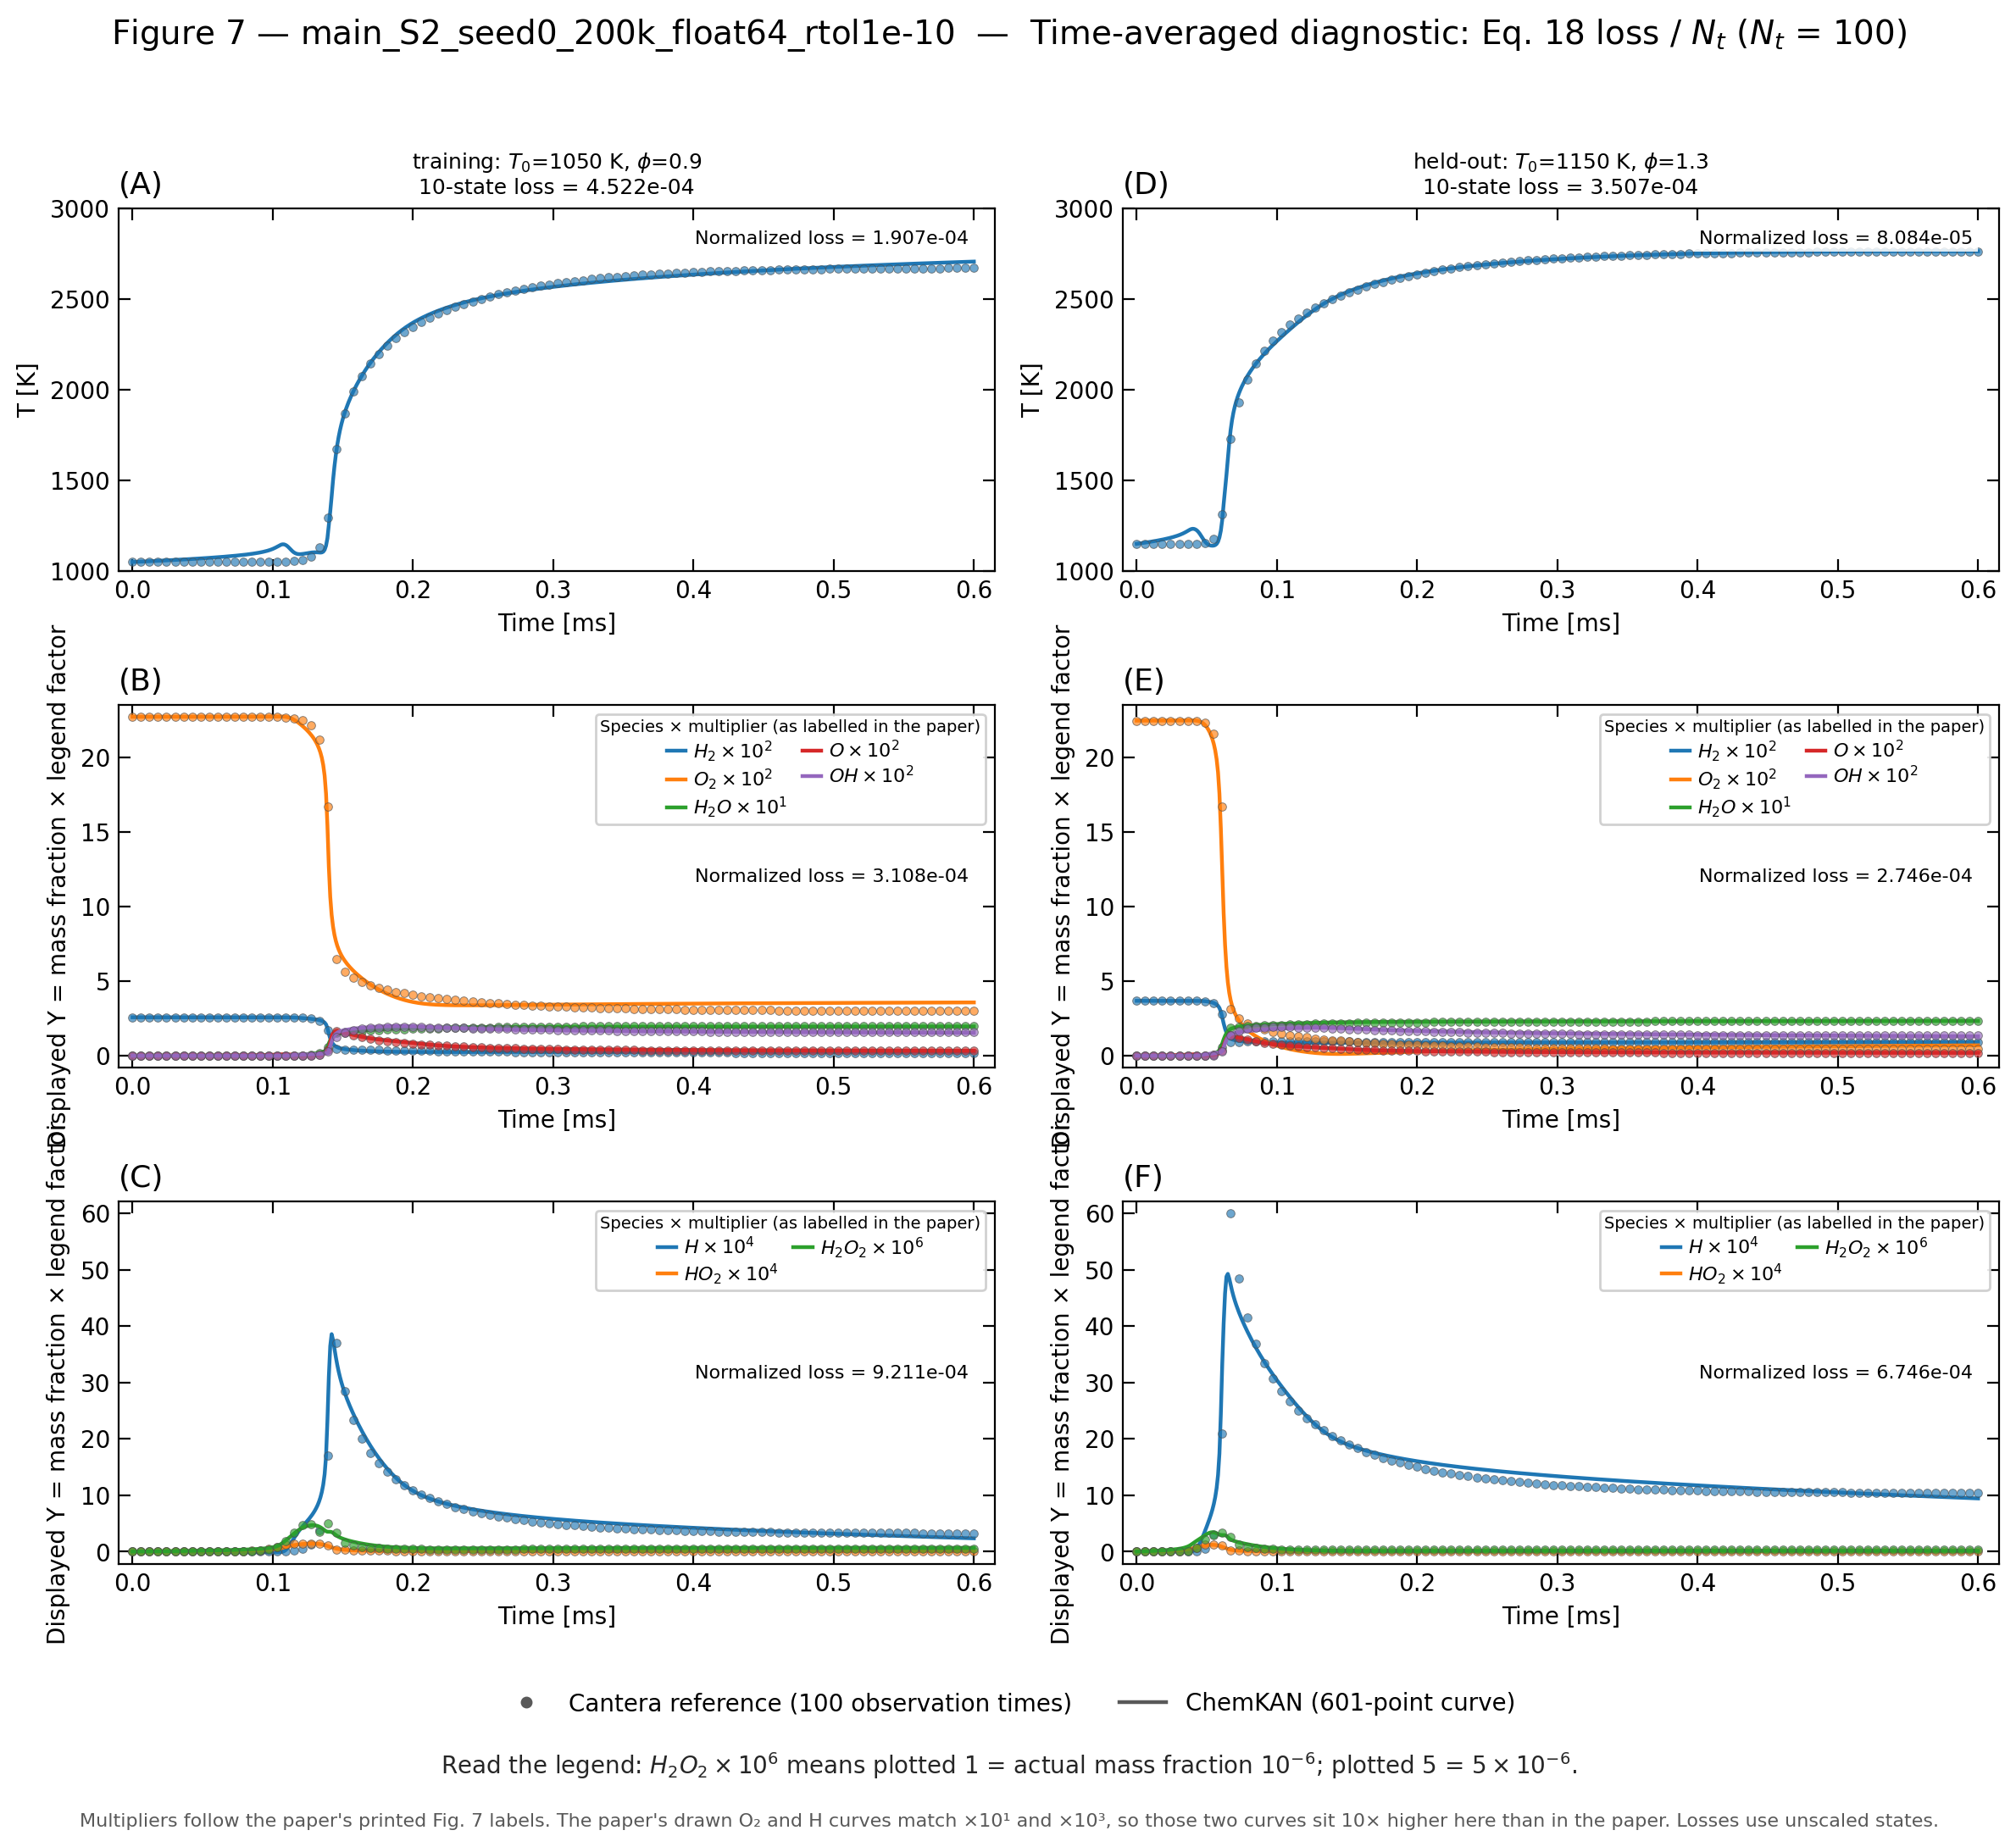
\includegraphics[width=0.98\textwidth]{ChemKAN_report_assets/hydrogen_fig07_200k_tight.png}
\caption{Hydrogen trajectories from the 200k Stage-2 checkpoint, re-evaluated in float64 with Tsit5 at \texttt{rtol}$=10^{-10}$ and \texttt{atol}$=10^{-12}$. The left column is the training condition $\phi=0.9$, $T_0=1050$~K; the right column is the held-out condition $\phi=1.3$, $T_0=1150$~K, corresponding to the paper's Figure~7.}
\label{fig:hydrogen_fig07}
\end{figure}

\begin{figure}[htbp]
\centering
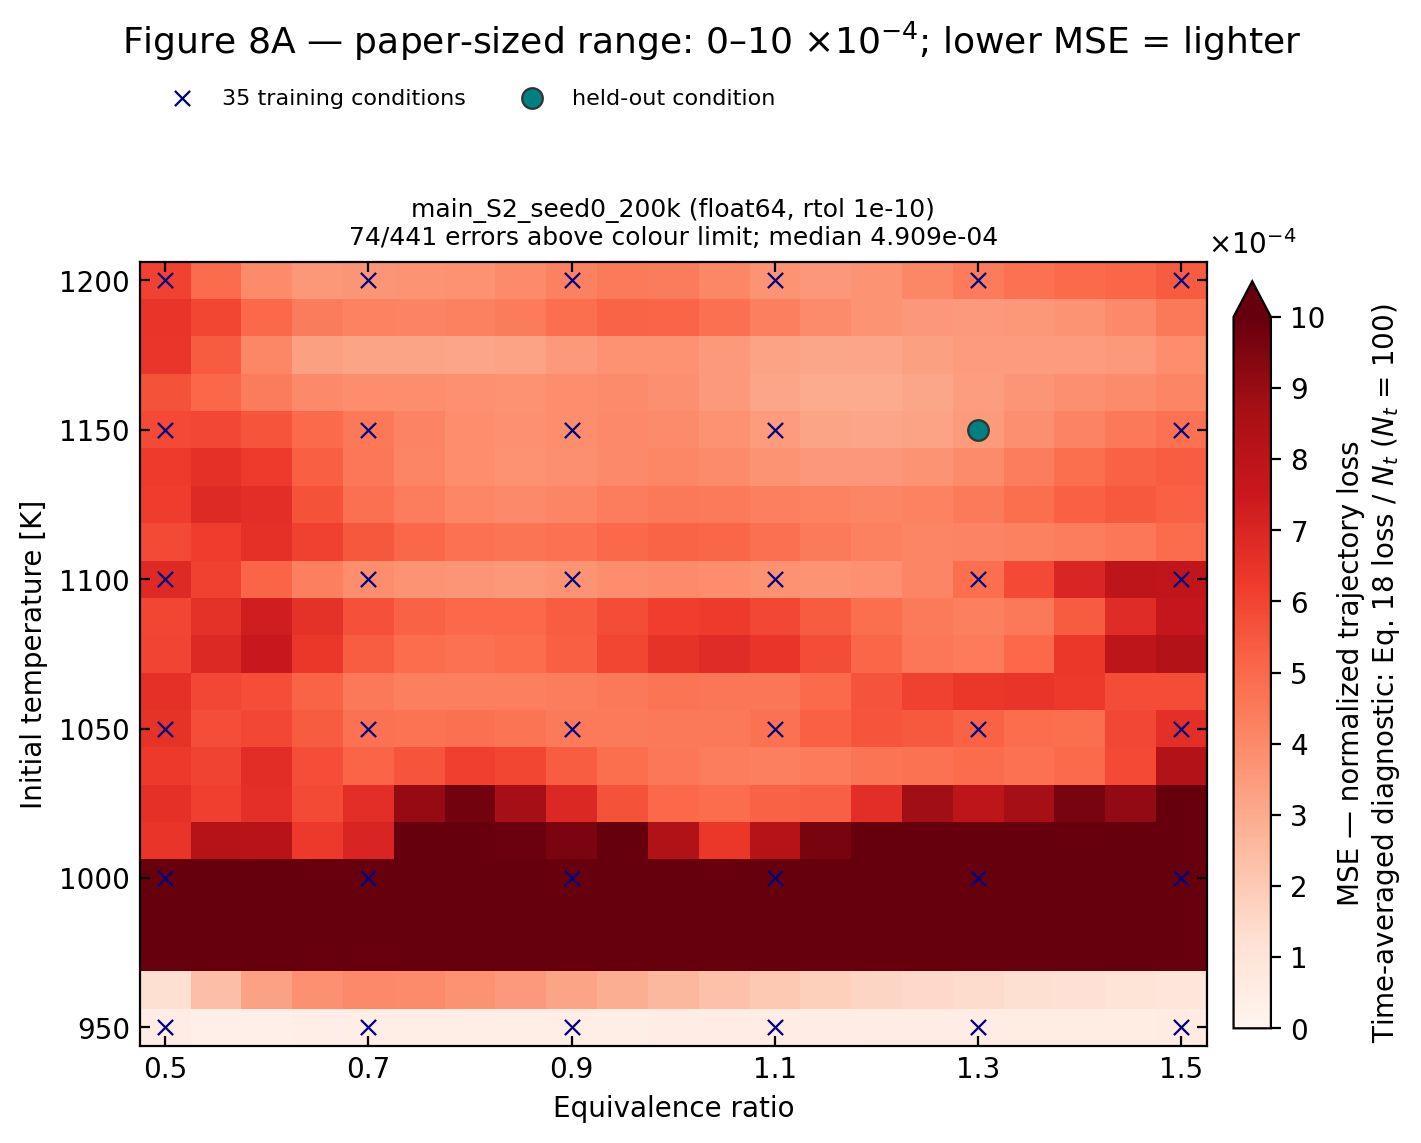
\includegraphics[width=0.72\textwidth]{ChemKAN_report_assets/hydrogen_fig08a_200k_tight.png}
\caption{Dense 441-condition generalization map for the 200k Stage-2 checkpoint, evaluated in float64 with Tsit5 at \texttt{rtol}$=10^{-10}$ and \texttt{atol}$=10^{-12}$. The plotted value is the normalized trajectory Eq.~(18) MSE divided by the 100 observation times.}
\label{fig:hydrogen_fig08a}
\end{figure}

\begin{figure}[htbp]
\centering
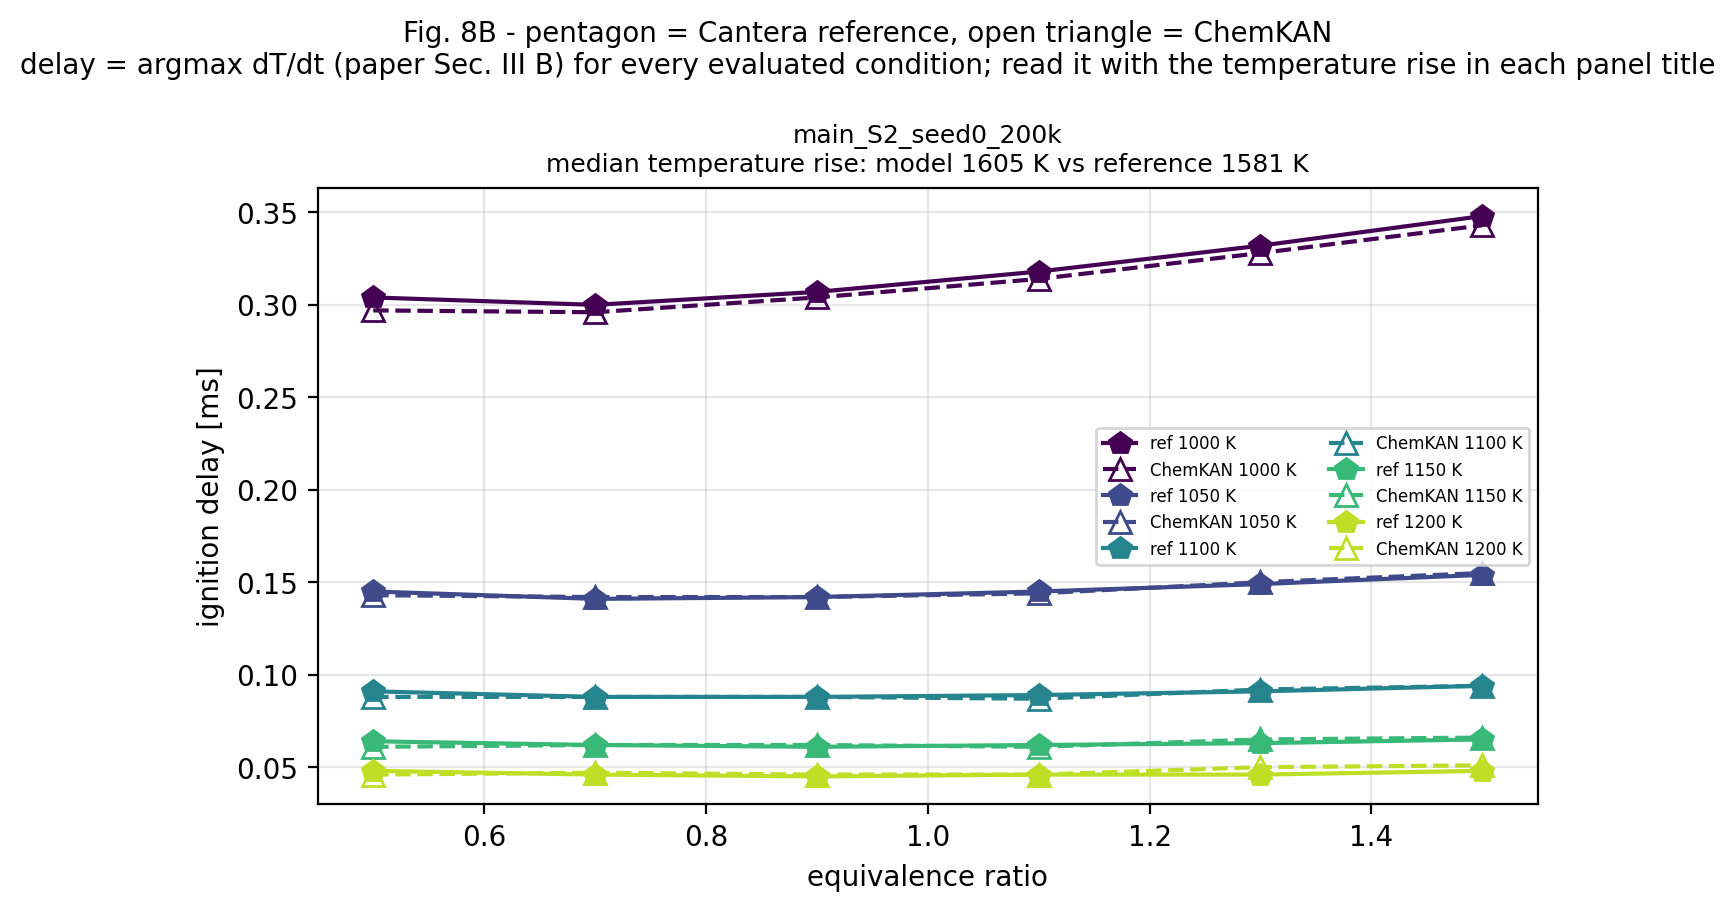
\includegraphics[width=0.82\textwidth]{ChemKAN_report_assets/hydrogen_fig08b_200k.png}
\caption{Ignition-delay comparison for the 200k Stage-2 checkpoint on the 30 conditions of the paper's Figure~8B ($T_0=1000,1050,1100,1150,1200$~K and all six equivalence ratios). Ignition delay is the time of maximum $\dd T/\dd t$.}
\label{fig:hydrogen_fig08b}
\end{figure}


The dense-grid evaluation reveals substantial differences
in accuracy across initial conditions. Although the median
time-averaged MSE over all 441 conditions is
$4.91\times10^{-4}$, errors increase considerably for
some conditions near the ignition-transition region.
For example, the median time-averaged MSE across
equivalence ratios at $T_0=987.5$~K is
$3.47\times10^{-2}$, compared with
$4.89\times10^{-4}$ at $T_0=1050$~K.

At $T_0=950$~K, where reference trajectories remain
approximately isothermal over the observation window,
the learned model produces small spurious temperature
increases for some conditions, but the corresponding
normalized trajectory errors remain comparatively low. These results indicate that predictive accuracy depends
on the initial thermochemical conditions. Further
inspection of individual trajectories is required to
distinguish ignition-timing errors from inaccuracies
in temperature and species dynamics.


\subsection{FSA validation and sensitivity-backend findings}

FSA was validated before it was used for scientific training. The validation suite covers: (i) the analytic scalar problem $\dd y/\dd t=\theta y$, whose sensitivity is known in closed form; (ii) biodiesel at initialized and trained parameters; (iii) hydrogen Stage~1 at initialized and trained parameters; and (iv) hydrogen Stage~2 at initialized and trained checkpoints under the tested thermodynamic initializations. It checks functional equivalence, FSA-versus-direct-autograd gradients under tolerance refinement, physical-state consistency, trajectory independence, production dtype, restart behavior, and selected finite-difference probes. The forward-sensitivity equation follows the standard formulation documented by SciMLSensitivity~\cite{SciMLSensitivityMath}.

\begin{table}[H]
\centering
\small
\caption{Forward Sensitivity Analysis validation summary.}
\label{tab:fsa_validation}
\begin{tabularx}{\textwidth}{@{}p{0.29\textwidth}p{0.21\textwidth}X@{}}
\toprule
\textbf{Validation item} & \textbf{Status} & \textbf{Meaning} \\
\midrule
Analytic ODE test & PASS & At tight tolerances, state/sensitivity and loss-gradient relative errors reach approximately $10^{-9}$. \\
Functional equivalence & PASS & The functional dynamics used for Jacobians reproduce the existing dynamics wrapper to numerical precision. \\
Gradient comparison & PASS under extended tolerance refinement & One hydrogen Stage-1 initial case required extending the tolerance ladder from $10^{-10}/10^{-12}$ to $10^{-12}/10^{-14}$; at the finer level both FSA and direct autograd converged and agreed under the same pre-defined thresholds. \\
State consistency / independence &
PASS after refinement amendment &
The augmented solve reproduces the
physical state, while batch-independence
checks passed at the amended finer
tolerance level. \\
Production dtype / resume & PASS & Float32 production runs remain finite and interrupted FSA runs reproduce uninterrupted optimizer/model/RNG state. \\
Finite differences & INCONCLUSIVE (optional) & Four selected probes pass; one very small correction-KAN gradient is dominated by cancellation and is not used as a blocking test. \\
\bottomrule
\end{tabularx}
\end{table}

The validation results support the correctness of the
implemented continuous FSA backend under the tested
configurations. The gradient-comparison and batch-independence checks required an additional
solver-tolerance refinement level (down to $\texttt{rtol}=10^{-12}$ and
$\texttt{atol}=10^{-14}$ in the affected comparison), as recorded in the historical
validation log. Some cases did not pass on the original refinement ladder.
The pre-defined gradient-error acceptance thresholds were unchanged.


A controlled biodiesel experiment provides an additional implementation-level comparison with the authors' released Julia example. Starting from the exact Julia initialization and using the same released-example data/settings, PyTorch FSA gives Julia-relative training-loss ratios of approximately 1.0001, 0.9999, and 0.997 at epochs 500, 2,000, and 5,000; the late training median is 0.94$\times$ Julia and the late validation median is 1.19$\times$ Julia. Direct differentiation through the PyTorch state-only solve remains about 1.5$\times$ above the Julia training loss in the same controlled comparison.

The released Julia biodiesel example uses \texttt{ForwardDiff.gradient} through \texttt{AutoTsit5(Rosenbro\\ck23)}, so derivative information participates in the differentiated solver computation. PyTorch FSA likewise integrates the sensitivity components with the physical state, whereas direct autograd integrates only the physical state and differentiates the solver computation graph afterwards. This offers a plausible numerical explanation for the closer PyTorch-FSA/Julia trajectory, but the project treats it as a hypothesis rather than a demonstrated causal mechanism.

The main hydrogen reproduction used direct
automatic differentiation, while the FSA
backend was validated independently and
evaluated in the controlled biodiesel comparison.


\subsection{Methane extension}


The methane-air oxidation experiment investigated
the transfer of ChemKAN to a larger chemical
system not included in the original study
\cite{Koenig_2025}. The model represented
52 species and temperature using GRI-Mech~3.0,
with 1,892 trainable parameters.

The methane Stage-1 training was initially
conducted on TU Wien's JupyterHub and resumed
on a local machine after epoch 28,000.
Stage~1 continued to approximately 54,800 epochs,
and the archived epoch-50,000 checkpoint was
used to initialize Stage~2. Stage~2 was
subsequently trained for 200,000 epochs. Because optimization was non-monotonic, archived
checkpoints were evaluated through complete
trajectory integrations. The epoch-180,000
checkpoint was selected using the mean
time-averaged MSE on the 35 training conditions,
without using the held-out condition.
The final epoch-200,000 checkpoint was
retained for comparison.


The selected model achieved a time-averaged
normalized MSE of $1.163\times10^{-3}$ on the
held-out condition
($T_0=1550$~K, $\phi=1.3$).
Across the complete 36-condition evaluation
grid, the median time-averaged MSE was
$9.94\times10^{-4}$. The model reproduced the overall ignition
events and major species trends. However,
some predicted temperature trajectories
developed a two-stage rise where the
reference temperature increased more
abruptly. Errors were also more pronounced
for certain radical and intermediate species. 

The final epoch-200,000 checkpoint was
evaluated separately and yielded a higher
median time-averaged MSE of
$1.47\times10^{-3}$ across the 36 conditions,
and $1.27\times10^{-3}$ for the held-out
condition. These results illustrate that
longer training did not monotonically
improve trajectory accuracy. The selected epoch-180,000 checkpoint is
evaluated visually in
Figure~\ref{fig:methane_heldout}, which
compares its held-out trajectory with the
Cantera reference, and in
Figure~\ref{fig:methane_error_grid_main},
which shows prediction errors across
the broader 441-condition grid.


\begin{figure}[htbp]
\centering
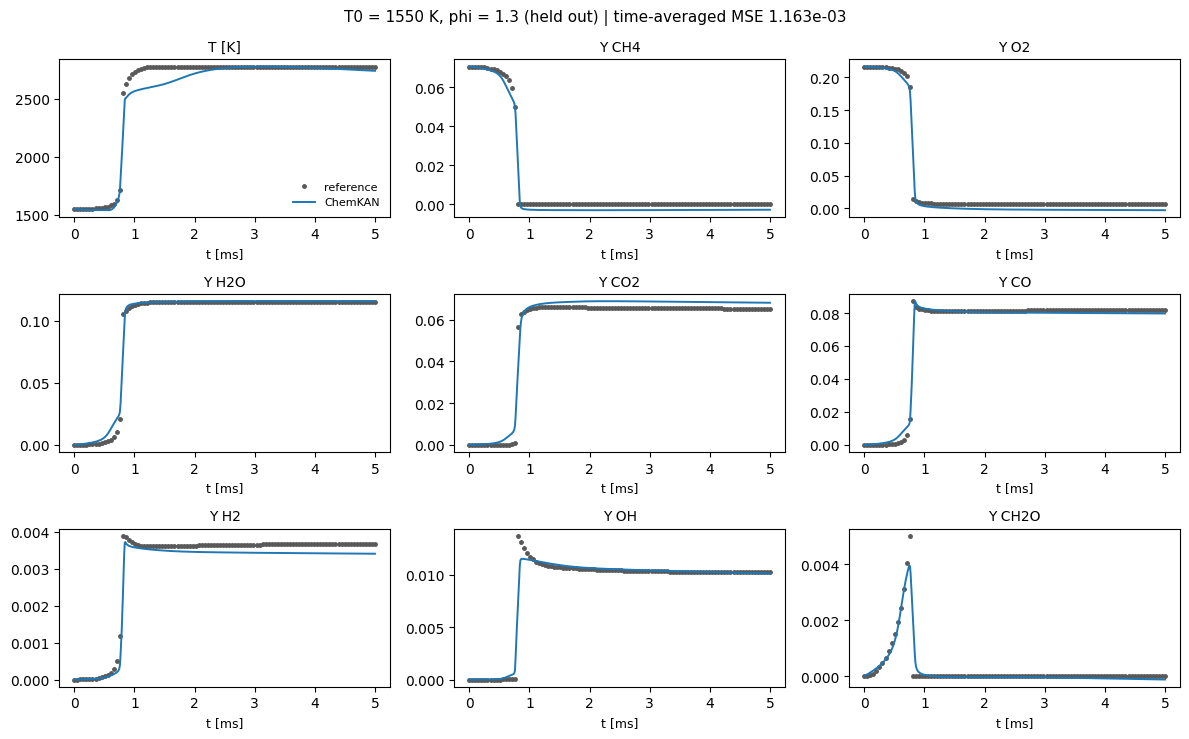
\includegraphics[width=0.97\textwidth]
{ChemKAN_report_assets/methane_180k_heldout_trajectory.png}
\caption{Methane-air oxidation on the held-out
condition $T_0=1550$~K, $\phi=1.3$, using the
selected epoch-180,000 Stage-2 checkpoint.
ChemKAN complete-rollout predictions are compared
with Cantera reference observations for temperature
and selected species. The time-averaged normalized
MSE is $1.163\times10^{-3}$.}
\label{fig:methane_heldout}
\end{figure}


\begin{figure}[htbp]
\centering
\begin{subfigure}[t]{0.49\textwidth}
    \centering
    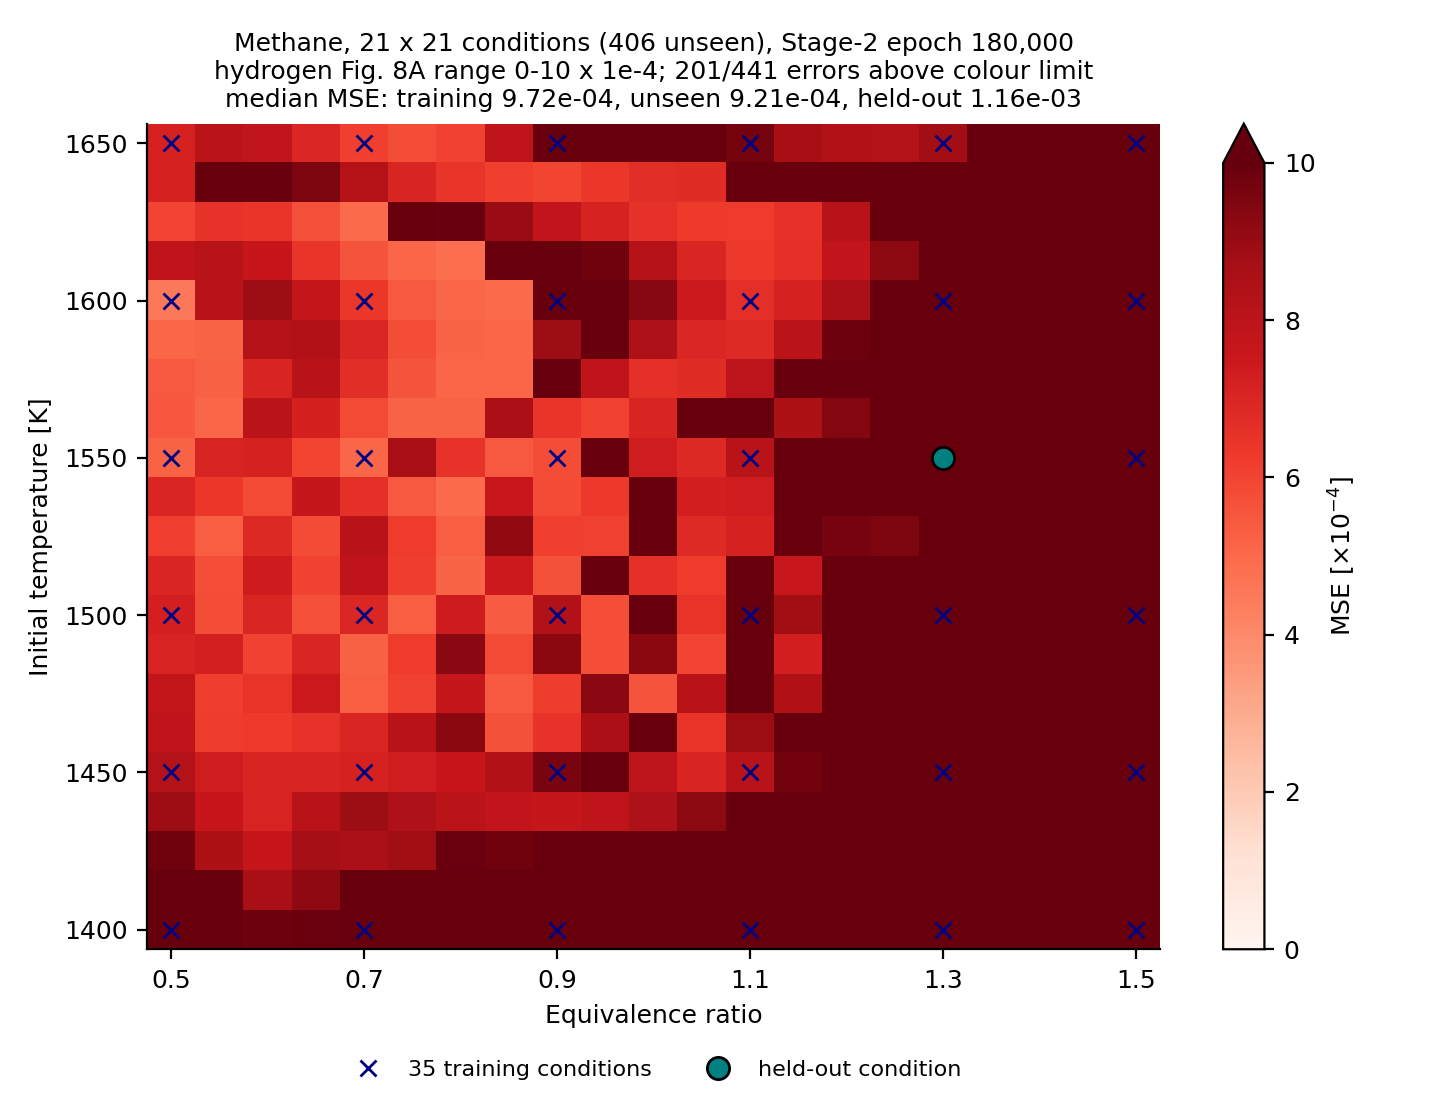
\includegraphics[width=\linewidth]
    {ChemKAN_report_assets/methane_generalization_441.png}
    \caption{Paper-style linear color scale.}
\end{subfigure}
\hfill
\begin{subfigure}[t]{0.49\textwidth}
    \centering
    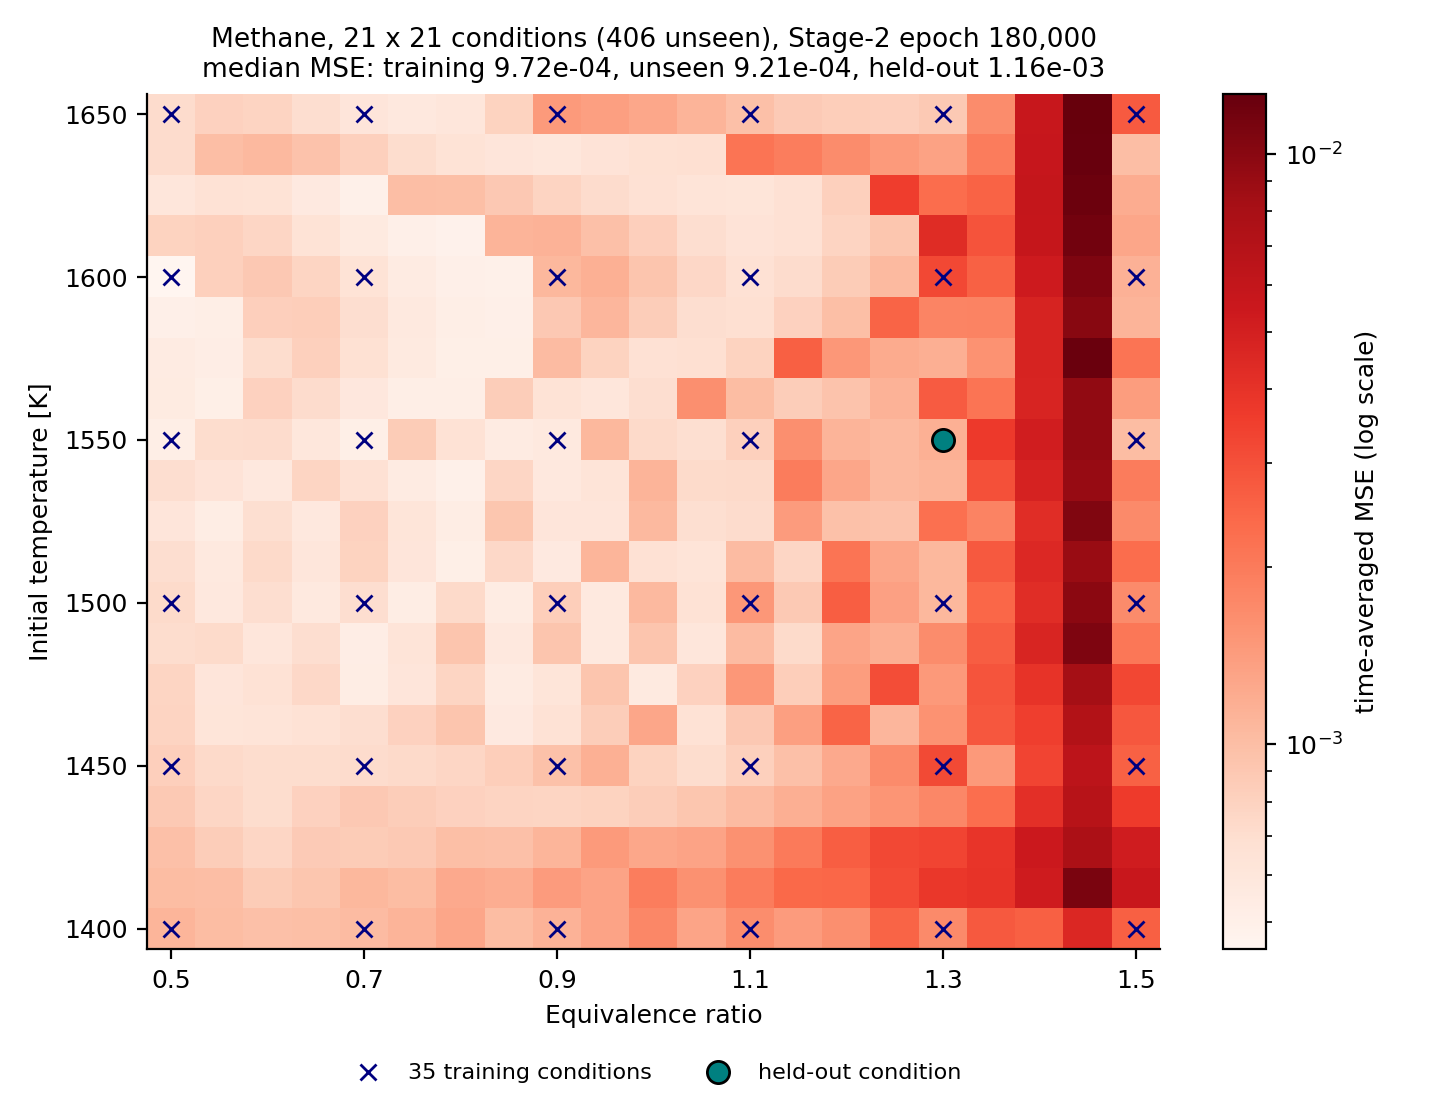
\includegraphics[width=\linewidth]
    {ChemKAN_report_assets/methane_generalization_441_full_range_log_scale.png}
    \caption{Full-range logarithmic color scale.}
\end{subfigure}
\caption{Generalization of the selected methane
Stage-2 epoch-180,000 checkpoint across 441 initial
conditions, comprising 35 training conditions
and 406 unseen conditions.
Time-averaged normalized MSE was evaluated over
100 observation times using float32 Tsit5 with
$\mathrm{rtol}=10^{-6}$ and
$\mathrm{atol}=10^{-8}$.
The left panel uses the paper-style color range
up to $10^{-3}$, while the right panel shows
the full error range logarithmically.}
\label{fig:methane_error_grid_main}
\end{figure}


The broader $21\times21$ initial-condition grid
contains 35 training and 406 unseen conditions.
The median time-averaged MSE is
$9.72\times10^{-4}$ for the training conditions
and $9.21\times10^{-4}$ for the unseen conditions. Although the model generalizes across much of the
investigated domain, higher errors occur around
$\phi=1.40$--$1.45$, where the maximum
time-averaged MSE reaches $1.27\times10^{-2}$.
The corresponding errors are particularly
pronounced for several low-concentration species. These observations show that the model's
generalization accuracy varies across the
initial-condition domain, despite the similar
median errors of the training and unseen groups.

Although Stage~2 was trained for 200,000 epochs,
the optimization had not clearly converged.
The median logged time-averaged MSE decreased
from $1.785\times10^{-3}$ over epochs
170,001--180,000 to $1.598\times10^{-3}$
over epochs 190,001--200,000. Further optimization or alternative Stage-1
checkpoint selection might affect the final
accuracy. These possibilities were not
investigated systematically, and the
200k training budget was retained for
consistency with the hydrogen experiments. 
The complete methane training history is
provided in Appendix~\ref{app:training_histories}.



\subsection{Computational efficiency}

A fair efficiency comparison must time the complete trajectory prediction task, not only a neural-network forward pass. ChemKAN still requires numerical ODE integration; it replaces the detailed chemical source-term function with a learned source-term model. For hydrogen and methane, the final benchmark therefore uses identical initial conditions, physical time horizons, and requested output grids for both Cantera and ChemKAN. Mechanism/model loading and data-file I/O are performed outside the timed region. Repeated measurements are used to report median latency, and accuracy is attached to every runtime result.

This is conceptually the same type of comparison used in ChemNODE. ChemNODE generated its reference/training trajectories with Cantera and then compared the time required to advance the learned model and the full detailed mechanism to steady state, reporting approximately $2.3\times$ speed-up~\cite{OWOYELE2022100118}. The original ChemKAN study reported approximately $2\times$ acceleration against detailed chemistry implemented with Arrhenius.jl~\cite{Koenig_2025,ji2021arrhenius}. The project-specific timing numbers are therefore interpreted as implementation- and hardware-specific measurements rather than as direct reproductions of those published speed-up factors.

Legacy local benchmarks were informative but are not used as the final efficiency claim because they were produced before the author-matched hydrogen configuration.


\paragraph{Benchmark implementation.}
Computational efficiency was measured for complete
trajectory integration, including per-trajectory
initialization and output conversion, while excluding
model loading, mechanism loading, compilation and file
I/O. The benchmark used one CPU thread on an Apple M1,
three warm-up calls, and 25 timed repetitions.
Single-trajectory latency and multi-condition
throughput were measured separately.


In addition to the primary PyTorch
implementation, an inference-only Julia
port was developed with AI-assisted code
generation using OrdinaryDiffEq.jl and
the Tsit5 solver
~\cite{Rackauckas-2017}. The Julia
implementation was not trained or
refitted; it used the same learned
parameters and normalization as the
PyTorch model. The two implementations
were compared numerically to verify
agreement of their predicted trajectories
before the runtime benchmarks were
conducted.

For hydrogen, the same 36 initial-value problems
were solved over 0.6~ms at 100 output times.
The detailed-chemistry references were Cantera and
Arrhenius.jl using the corresponding hydrogen
mechanism. For biodiesel, the learned dynamics were
compared against the known reaction equations using
SciPy LSODA and Julia-based numerical integration.


\begin{table}[htbp]
\centering
\small
\caption{Single-trajectory median inference latency
on an Apple M1 CPU (one thread, 100 output points).
The selected PyTorch-trained ChemKAN parameters
were used in both execution environments.
Detailed-chemistry references were evaluated
at their data-generation tolerances.}
\label{tab:efficiency}
\begin{tabular}{@{}lrrrr@{}}
\toprule
\textbf{System} &
\textbf{PyTorch} &
\textbf{Julia} &
\textbf{Python ref.} &
\textbf{Julia ref.} \\
& \multicolumn{4}{c}{\textbf{Median latency (ms)}} \\
\midrule
Hydrogen  & 111.51 & 1.60 & 3.94 & 10.07 \\
Methane   & 117.05 & 9.93 & 39.57 & 134.29 \\
Biodiesel & 67.17  & 0.69 & 1.20 & 0.20 \\
\bottomrule
\end{tabular}
\end{table}


The combustion ChemKAN integrations used
$\mathrm{rtol}=10^{-6}$ and
$\mathrm{atol}=10^{-8}$, whereas the detailed
chemistry references used the tighter
data-generation tolerances
($10^{-9}/10^{-15}$).
The biodiesel comparison used its separately
documented tight evaluation settings.
Consequently, the measured speed-ups apply
to these numerical configurations and do
not constitute comparisons at guaranteed
equal numerical error.

The implementation language substantially affected
computational efficiency. For hydrogen, the Julia
ChemKAN inference implementation achieved
approximately $2.5\times$ lower latency than
Cantera and $6.3\times$ lower latency than
Arrhenius.jl. For methane, the corresponding
speed-ups increased to approximately $4.0\times$
and $13.5\times$.

In contrast, PyTorch ChemKAN required
approximately 111.5~ms and 117.0~ms per trajectory
for hydrogen and methane, respectively, and was
slower than Cantera in both cases.

The Julia implementation used weights exported
from the PyTorch-trained models without
retraining. Agreement between the two inference
implementations was independently verified.
Thus, the runtime differences are associated
with the numerical and software execution
environment rather than with different
learned model parameters. For biodiesel, which contains only three
reactions, Julia's direct integration of the
known kinetics was faster than Julia ChemKAN
at the tight evaluation tolerance.

These results illustrate that the efficiency
of a neural ODE surrogate depends on both
chemical-system complexity and the implementation
of the learned right-hand side. 
Figure~\ref{fig:runtime_accuracy} summarizes
the relationship between inference latency
and prediction accuracy across the evaluated
chemical systems and numerical configurations.


\begin{figure}[htbp]
\centering
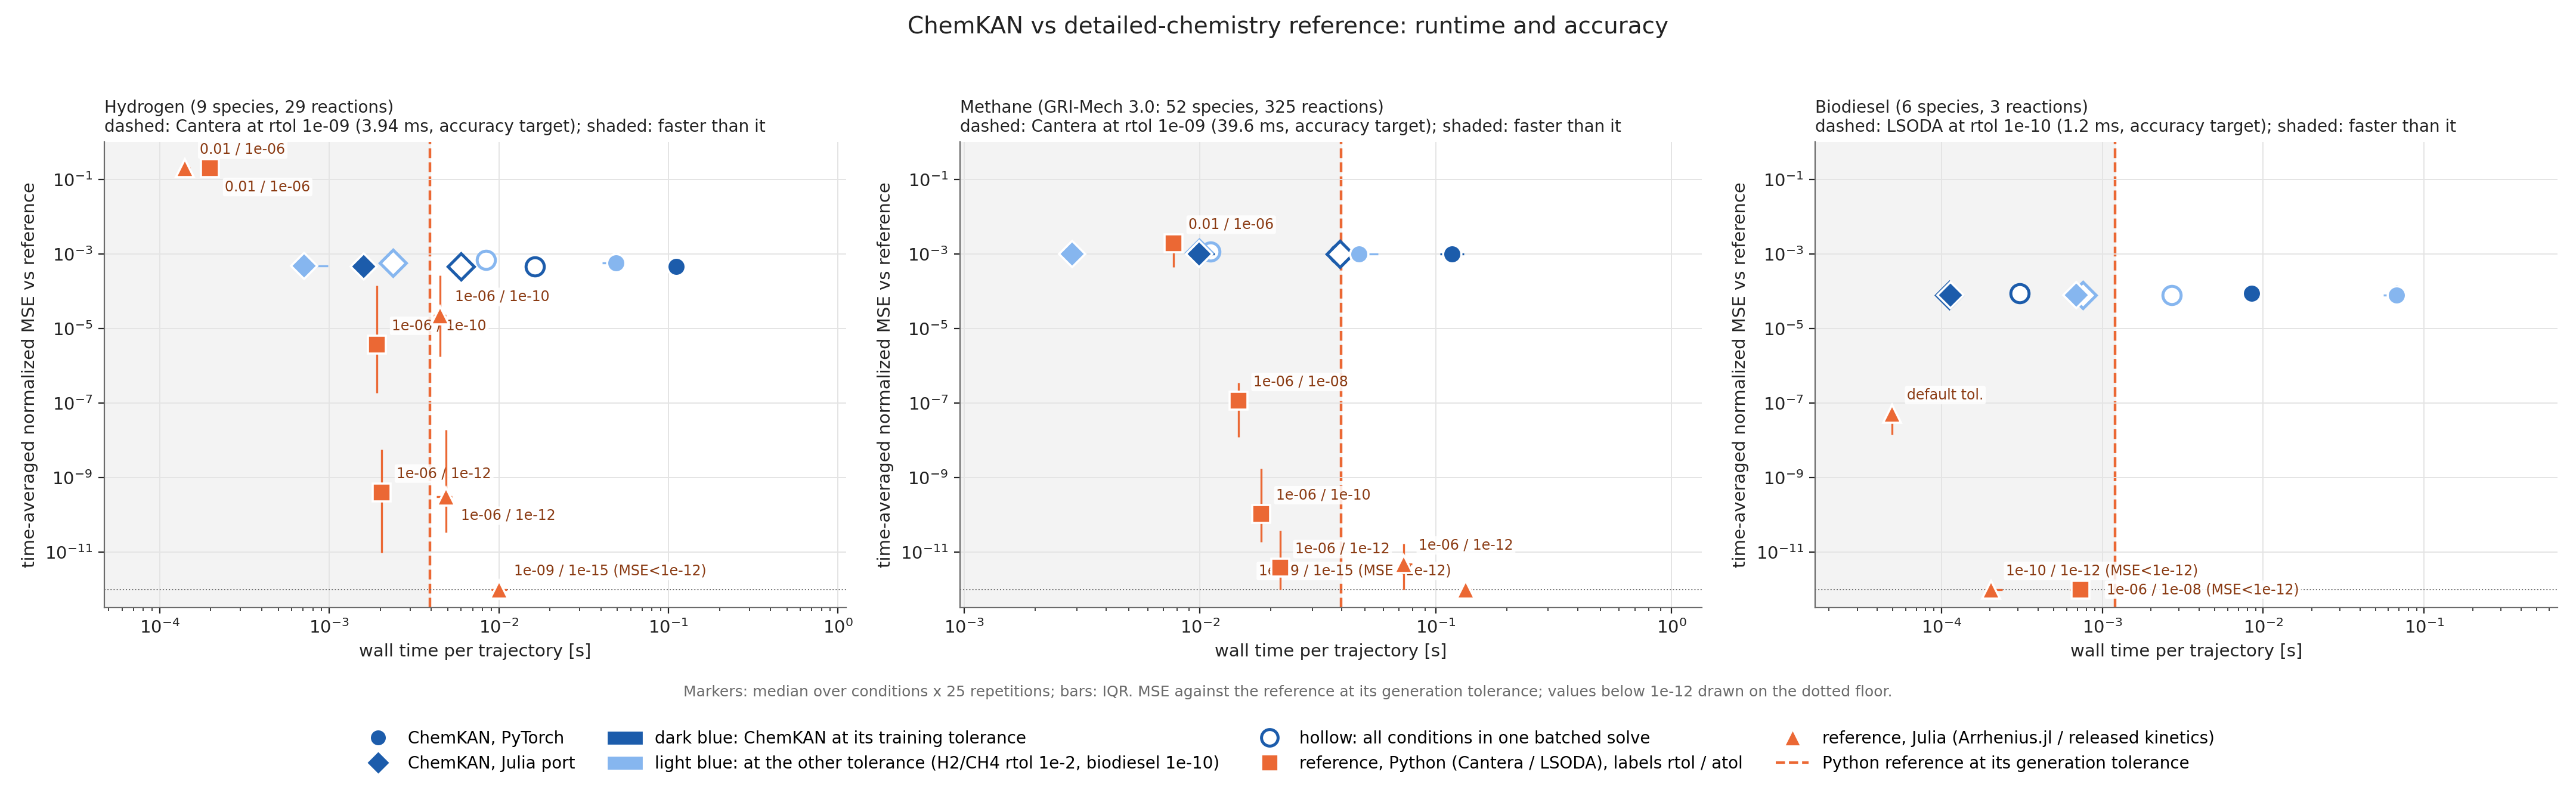
\includegraphics[width=\textwidth]{ChemKAN_report_assets/runtime_vs_accuracy.png}
\caption{Inference latency and time-averaged
normalized trajectory MSE for the three chemical
systems, comparing PyTorch and Julia ChemKAN
with their numerical reference methods under
different solver tolerances. Markers indicate
median measurements and error bars the
interquartile ranges.}
\label{fig:runtime_accuracy}
\end{figure}



\subsection{Interpretability}

The learned biodiesel ChemKAN was examined through
its univariate edge activation functions and through
the behavior of the complete learned kinetic
right-hand side. The analysis used the final
156-parameter noise-free biodiesel checkpoint.
No additional training was performed.

The first-layer KAN functions provide a
decomposition of how individual normalized
state variables contribute to the hidden
representation. Figure~\ref{fig:interpretability_edges}
shows the learned univariate functions connecting
the six species concentrations and temperature
to the four hidden nodes.

These functions can be inspected individually,
but their effects on the predicted reaction
rates also depend on the subsequent LeanKAN
layer. Therefore, individual edge shapes
should not be interpreted directly as
chemical reaction laws.

\begin{figure}[htbp]
\hspace{-1cm}
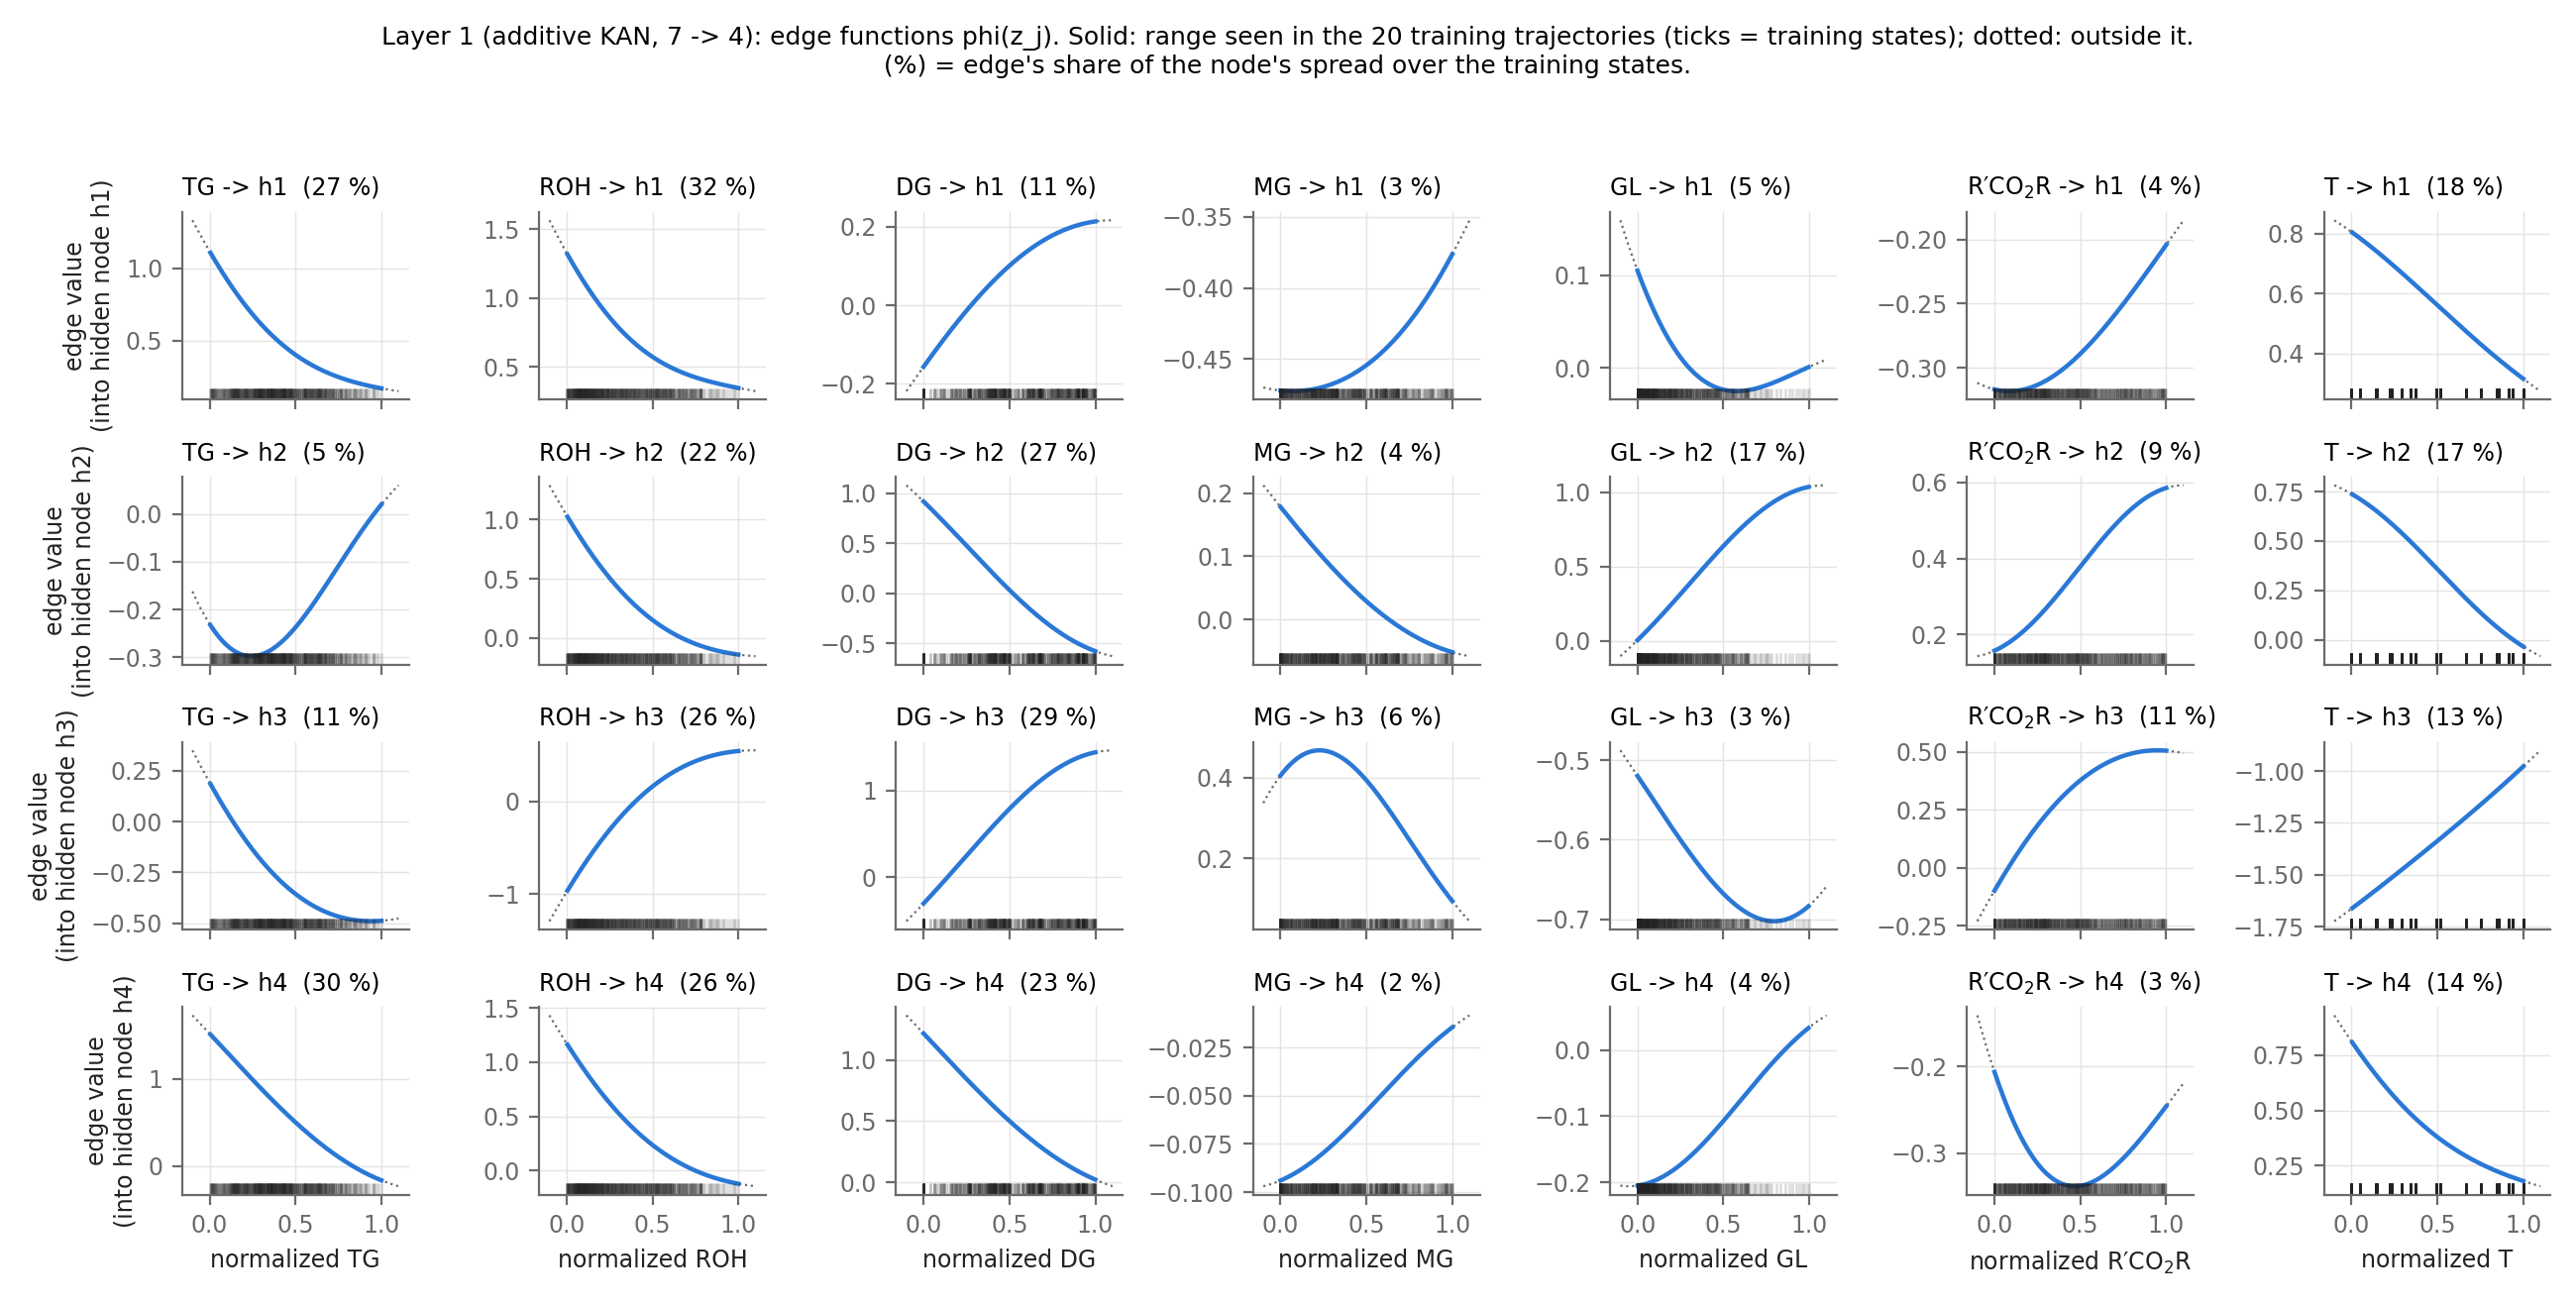
\includegraphics[width=1.10\textwidth]
{ChemKAN_report_assets/interpretability_biodiesel_edges_layer1.png}
\caption{Learned first-layer univariate edge
activation functions of the final noise-free
biodiesel ChemKAN, evaluated over the observed
training-domain input ranges.}
\label{fig:interpretability_edges}
\end{figure}


\begin{figure}[htbp]
\hspace{-1cm}
\centering
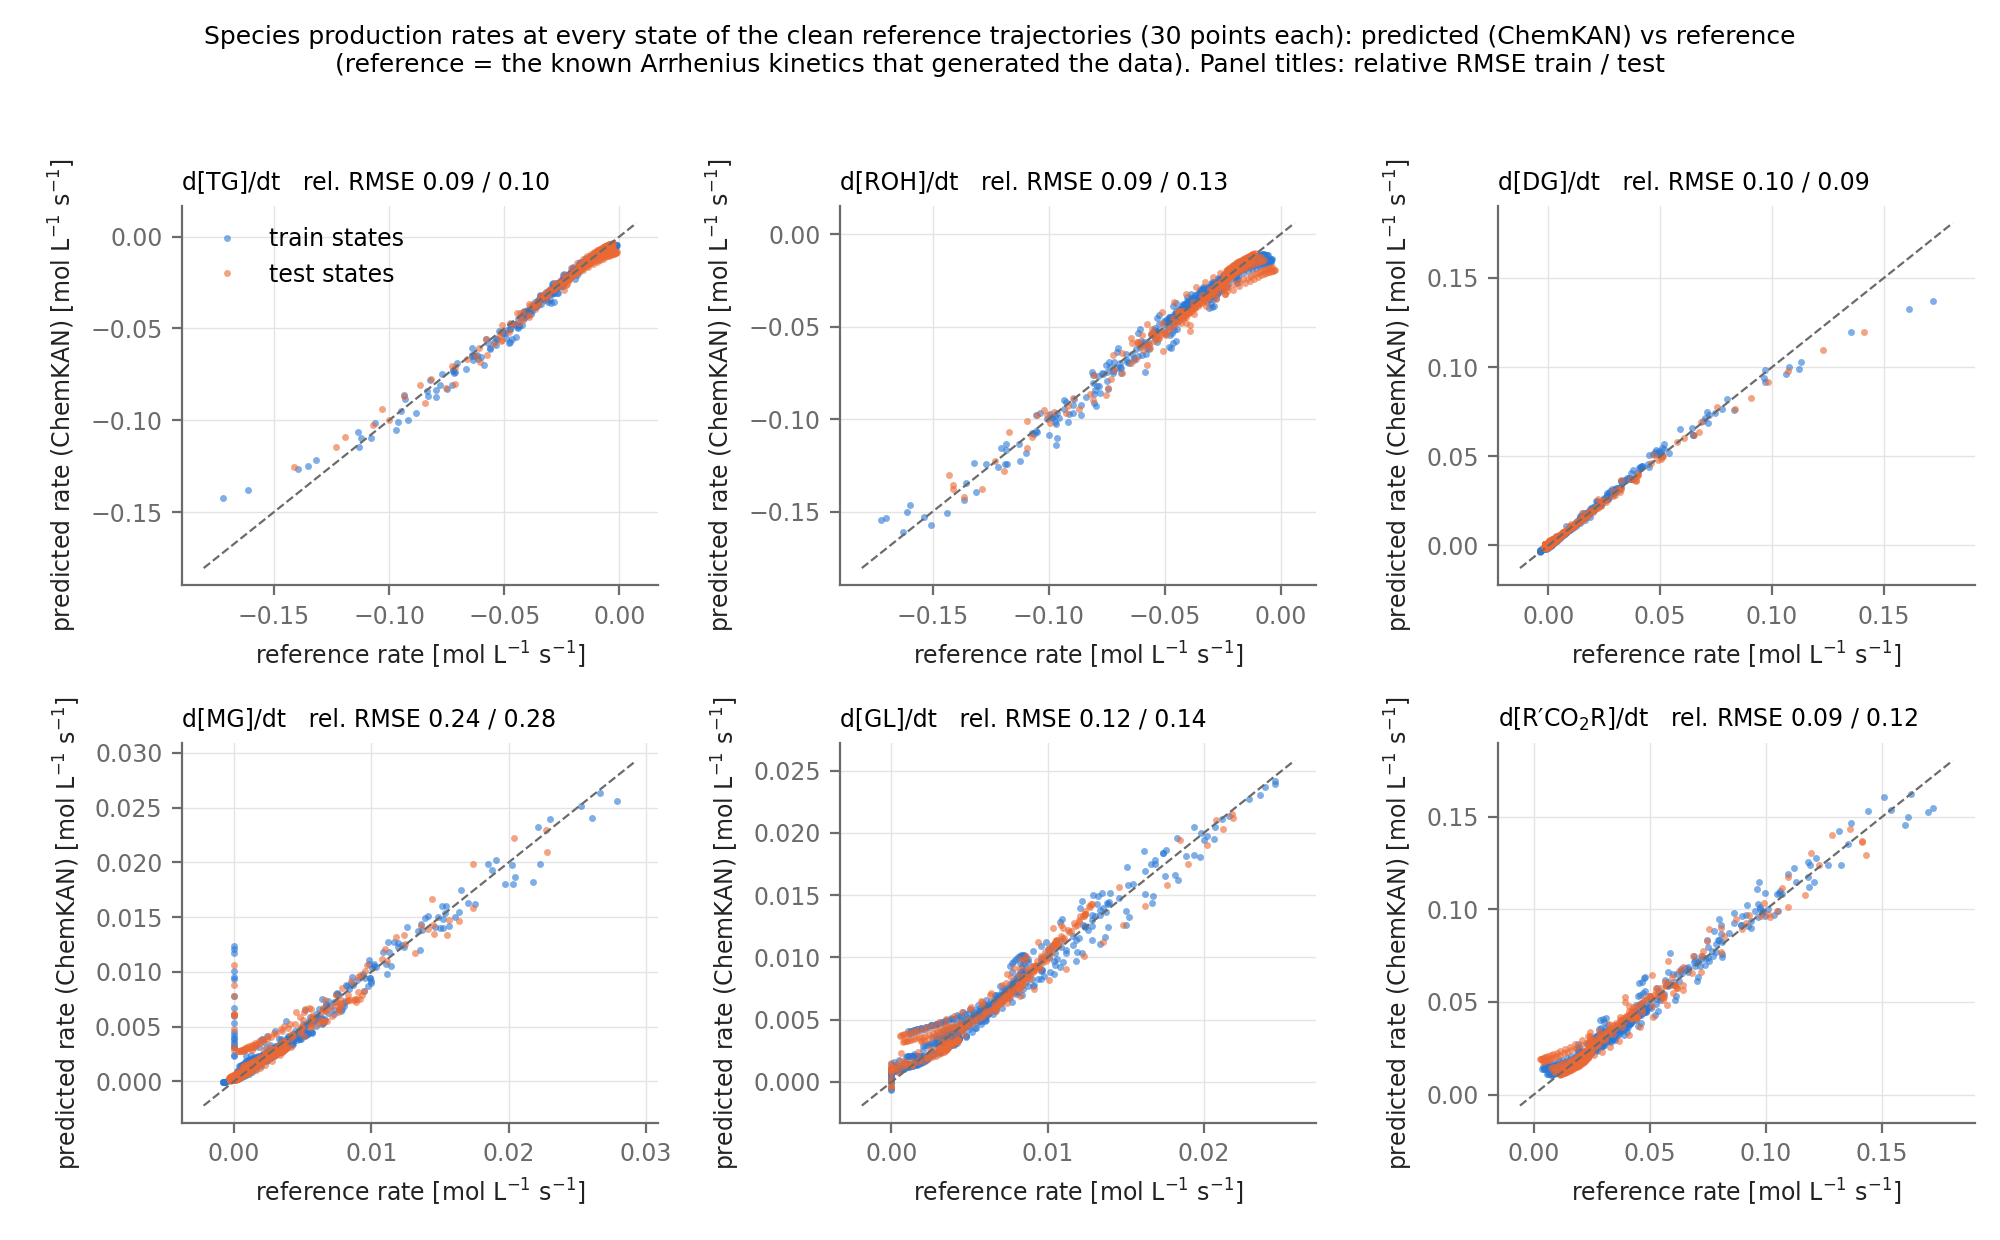
\includegraphics[
    width=0.97\textwidth,
    keepaspectratio
]{ChemKAN_report_assets/interpretability_biodiesel_rate_parity.png}
\caption{Biodiesel species production rates predicted
by the complete learned ChemKAN and the known
Arrhenius kinetics at 600 training and 300 held-out
reference states. The dashed diagonal represents
perfect agreement. Relative RMSE values are shown
for each species, separately for training and
held-out states.}
\label{fig:interpretability_rate_parity}
\end{figure}


For each species, the relative root-mean-square
error of the predicted production rate is
defined as
\begin{equation}
\mathrm{rRMSE}_k =
\frac{
\sqrt{
\frac{1}{N}
\sum_{i=1}^{N}
\left(
\dot{u}_{k,i}^{\mathrm{pred}}
-
\dot{u}_{k,i}^{\mathrm{ref}}
\right)^2
}
}{
\sqrt{
\frac{1}{N}
\sum_{i=1}^{N}
\left(
\dot{u}_{k,i}^{\mathrm{ref}}
\right)^2
}
}.
\end{equation}
The metric is evaluated separately on
training and held-out reference states.

Figure~\ref{fig:interpretability_rate_parity}
compares the complete learned ChemKAN kinetic
right-hand side with the known Arrhenius kinetics
at 600 training and 300 held-out states sampled
from clean reference trajectories. The rates are
evaluated at the same states, without integrating
new trajectories or varying the inputs.

The predicted rates generally follow the reference
rates for TG, ROH, DG, GL, and R'CO$_{2}$R,
with relative RMSE between 0.09 and 0.14 across
the training and held-out sets. The largest
discrepancy occurs for MG (0.24 training and
0.28 held-out relative RMSE). In particular,
ChemKAN predicts positive MG production rates
at some states where the reference production
rate is approximately zero.

These results indicate that ChemKAN approximates
most biodiesel source terms well at the sampled
reference states, although discrepancies remain
for some species. The learned edge functions
allow inspection of the model's functional
structure, while the rate comparison provides
a quantitative assessment of its agreement
with known kinetics. However, this does not
establish that the individual learned functions
correspond to specific chemical reactions.

Additional read-only interpretability diagnostics
were also generated for hydrogen and methane.
The detailed discussion here focuses on
biodiesel because its known, compact
Arrhenius mechanism permits direct validation
of the learned kinetic rates. A systematic
cross-system interpretability comparison was
not undertaken.



\subsection{Evaluation against proposal success criteria}

\begin{table}[H]
\centering
\small
\caption{Evaluation against the five success
criteria defined in the approved proposal.}
\label{tab:success_criteria}
\begin{tabularx}{\textwidth}{@{}p{0.30\textwidth}X@{}}
\toprule
\textbf{Success criterion} &
\textbf{Experimental evidence and observations} \\
\midrule

Implementation &
An independent PyTorch ChemKAN implementation
includes the kinetic core, thermodynamic
superstructure, two-stage training, direct
autograd, and a validated continuous-FSA backend. \\

Reproduction &
Biodiesel reproduces several reported noise
robustness trends under the clarified protocol.
The 200k hydrogen model predicts the designated
held-out condition with time-averaged MSE
$3.507\times10^{-4}$ and has a median absolute
ignition-delay error of 1.36\% on the Figure~8B
conditions. Some quantitative discrepancies
remain across initial conditions.
The comparison with published hydrogen
MSE ranges is sensitive to the loss
normalization convention, and agreement
is not uniform across the reconstructed
initial-condition grid.\\

Extension &
ChemKAN was extended to methane-air oxidation
using GRI-Mech~3.0. Stage~2 training reached
200,000 epochs, with the 180k checkpoint selected
for evaluation. The held-out time-averaged MSE
was $1.163\times10^{-3}$.
The Julia inference port achieved approximately
$4.0\times$ acceleration relative to Cantera
under the measured configuration. \\

Comparative analysis &
DeepONet was reconstructed and compared with
ChemKAN under controlled biodiesel experiments.
Published ChemNODE results were used for
context. Computational efficiency was measured
against detailed numerical chemistry in Python
and Julia. See Table~\ref{tab:efficiency}. \\

Interpretability &

The learned KAN edge functions were visualized
and the complete biodiesel kinetic right-hand
side was compared with the known Arrhenius rates.
The model approximated most species production
rates at sampled reference states, although
larger discrepancies remained for MG.
Individual learned functions were not uniquely
identified with specific chemical reactions.\\

\bottomrule
\end{tabularx}
\end{table}

\section{Discussion and State-of-the-Art Comparison}

\subsection{RQ1: Reproducibility of ChemKAN}

The independent PyTorch implementation reproduces the central behavior of both original case studies, but exact quantitative reproduction could not be obtained from the paper text alone. In the first paper-only implementation, extensive ablations reduced some discrepancies but the hydrogen thermodynamic stage still failed to reproduce temperature ignition reliably and biodiesel losses remained above the reported levels. The later author clarification and released biodiesel source resolved several settings that materially changed the reproduction~\cite{ChemKANAuthors2026,ChemKANRepo2026}.

For biodiesel, the revised setup closely reproduces the reported noise-floor behavior and approximately two-fold clean-test degradation at 15\% noise, while the reconstructed neural-scaling and DeepONet results remain more sensitive. For hydrogen, the 200k Stage-2 checkpoint reproduces ignition timing and the main trajectory behavior with a dense-grid median time-averaged MSE of $4.91\times10^{-4}$ and 1.36\% median absolute ignition-delay error on the Figure~8B conditions. The reproduction is therefore best described claim by claim rather than as a single binary success/failure result.


\subsection{RQ2: Transfer to methane-air oxidation}

The methane extension demonstrated that the ChemKAN
architecture can be applied to a chemical system
substantially larger than the hydrogen benchmark.
Using 1,892 trainable parameters, the selected
model learned the principal ignition and species
trajectories of the GRI-Mech~3.0 system.

For the held-out initial condition, the model
achieved a time-averaged normalized MSE of
$1.163\times10^{-3}$. Across the 36 investigated
initial conditions, the median error was
$9.94\times10^{-4}$. The model reproduced the
overall ignition behavior, although discrepancies
remained in transient temperature profiles
and several intermediate-species trajectories.
The broader 441-condition evaluation further
demonstrated generalization to unseen
initial-condition combinations, with a median
time-averaged MSE of $9.21\times10^{-4}$
across the 406 unseen conditions.


Computational efficiency depended strongly on the
execution environment. The Julia inference port
was approximately four times faster than Cantera
and 13.5 times faster than Arrhenius.jl under the
measured configurations. The PyTorch implementation
was slower than Cantera for individual trajectories.

The extension therefore provides evidence of
transferability to a larger chemical system,
while also demonstrating that training stability,
physical fidelity, and practical acceleration
must be evaluated separately.



\subsection{RQ3: Comparison with neural and numerical references}

DeepONet predicts the future state directly from
the initial condition and time, avoiding ODE
integration during inference~\cite{lu2019deeponet}.
The original ChemKAN study used DeepONet as
the neural baseline for biodiesel production
and reported stronger overfitting under noisy
training observations~\cite{Koenig_2025}.
In this project, the 308-parameter DeepONet
architecture was reconstructed using the
published model size and clarifications
from the authors. Because the exact activation
functions and optimization settings were
not fully specified, the selected tanh
reconstruction is treated as a
behavior-matching implementation rather
than an exact recovery of the authors'
original DeepONet.

The results in Figure~\ref{fig:biodiesel_noise}
and Table~\ref{tab:biodiesel_summary} show
that the selected 308-parameter DeepONet
achieved comparable or lower clean-test MSE
than the 156-parameter ChemKAN at several
lower observation-noise levels. At 10\%
and 15\% noise, however, ChemKAN achieved
approximately 2.7-fold lower clean-test MSE.
The single-seed reproduction therefore
supports a relative advantage for ChemKAN
at higher noise levels, but not uniform
superiority across all investigated noise
levels.

ChemNODE provides a published neural-ODE
baseline for hydrogen-air combustion.
Like ChemKAN, it learns chemical source
terms that are integrated to obtain
thermochemical trajectories. However,
ChemNODE uses separately trained neural
networks for individual thermochemical
variables, whereas ChemKAN combines
the kinetic and thermodynamic components
within a single chemistry-specific
KAN architecture. ChemNODE modeled six
species and temperature, while the hydrogen
ChemKAN models represent nine species and
temperature~\cite{OWOYELE2022100118,Koenig_2025}.

\begin{table}[htbp]
\centering
\small
\caption{Architectural and computational
comparison of ChemNODE and hydrogen ChemKAN.
Published speed-ups and measurements from
this work use different hardware, reference
solvers, and timing protocols and are not
directly comparable across studies.}
\label{tab:chemnode_comparison}
\begin{tabularx}{\textwidth}{@{}lccXXr@{}}
\toprule
\textbf{Model} &
\textbf{Nets} &
\textbf{Params} &
\textbf{States} &
\textbf{Reference} &
\textbf{Speed-up} \\
\midrule
ChemNODE (published)
& 7 & 637$^{a}$
& 6 species + $T$
& Detailed chemistry
& $2.3\times$ \\

ChemKAN (published)
& 1 & 344
& 9 species + $T$
& Arrhenius.jl
& $2.0\times$ \\

ChemKAN (PyTorch)
& 1 & 344
& 9 species + $T$
& Cantera
& $0.035\times$ \\

ChemKAN (Julia)
& 1 & 344
& 9 species + $T$
& Cantera
& $2.5\times$ \\

ChemKAN (Julia)
& 1 & 344
& 9 species + $T$
& Arrhenius.jl
& $6.3\times$ \\
\bottomrule
\end{tabularx}

\smallskip
\raggedright\footnotesize
$^{a}$ ChemNODE parameter count estimated
in~\cite{Koenig_2025} using standard MLP
parameterizations (seven networks with
91 parameters each).
\end{table}

ChemNODE achieved approximately $2.3\times$
acceleration over the detailed hydrogen-air
mechanism for integration to steady state
~\cite{OWOYELE2022100118}. The original
ChemKAN paper reported approximately
$2.0\times$ acceleration using Arrhenius.jl
as the detailed-chemistry reference
~\cite{Koenig_2025}. These published
results are included for architectural
and methodological context; ChemNODE was
not independently retrained or benchmarked
in this project.

The primary ChemKAN reproduction was
implemented and trained in PyTorch.
Under the local hydrogen inference
benchmark, the PyTorch implementation
required approximately 111.5~ms per
trajectory, compared with 3.94~ms
for Cantera. Thus, despite reproducing
the principal combustion behavior,
the direct PyTorch implementation
did not achieve the computational
acceleration reported in the original
ChemKAN study.

To investigate the influence of the
execution environment, an inference-only
implementation was subsequently developed
in Julia using the parameters learned
in PyTorch. No additional model training
or parameter fitting was performed.
Agreement between the PyTorch and Julia
predictions was verified before benchmarking.
The Julia port required approximately
1.60~ms per hydrogen trajectory,
corresponding to $2.5\times$ acceleration
over Cantera and $6.3\times$ over
Arrhenius.jl under the evaluated
configurations.

The local benchmarks therefore show
that inference efficiency depends
substantially on the numerical
implementation, even when the learned
parameters remain unchanged.
Nevertheless, the published ChemNODE
and ChemKAN speed-ups cannot be
interpreted as a direct performance
ranking against the present results,
because the numerical references,
hardware, and timing tasks differ.

The effect of mechanism complexity was
also evident across the investigated
systems. For the three-reaction biodiesel
system, direct Julia integration of
the known kinetics remained faster
than Julia ChemKAN. In contrast,
the Julia ChemKAN ports achieved
acceleration over detailed chemistry
for hydrogen and methane, with larger
measured speed-ups for methane.
These findings suggest that potential
computational savings depend on both
chemical-system complexity and the
execution environment, rather than
on neural-network parameter count alone.


\subsection{Reproducibility lessons}

The project shows that scientific machine-learning reproduction requires source-level provenance in addition to architectural similarity. Several examples materially affected the experiments: the printed biodiesel reaction ordering differs from the released code; printed Eq.~(18) sums over time while the released Julia example uses time-averaged \texttt{Flux.mse}; the paper describes a Swish base activation while the authors clarified that the final models did not use it; the paper text omits $\phi=0.5$ from the hydrogen list although the 36-condition design includes it; and the released biodiesel example uses \texttt{AutoTsit5(Rosenbrock23)} rather than only Tsit5. The hydrogen clarification additionally supplied the 100-point grid, dense Stage-1 temperature interpolation, $10^{-5}$ thermodynamic initialization, and the $10^5$--$2\times10^5$ training budget.

Where later source material or author clarification resolves a discrepancy, the final reproduction adopts the directly supported setting and states its provenance instead of treating it as a convention introduced by this project. Earlier paper-only results are retained because they show which details were necessary to obtain the later reproduction.

The FSA comparison provides a second numerical lesson. Matching architecture, data, initialization, optimizer, and nominal tolerances does not by itself guarantee an identical optimization trajectory when the sensitivity method changes the variables included in the adaptive solve. The close PyTorch-FSA/Julia training trajectory is therefore reported as evidence about numerical implementation sensitivity, while the proposed error-control explanation remains explicitly a hypothesis.

The cross-language inference comparison also shows
that numerical and software implementation choices
can dominate the measured computational efficiency
of a small learned surrogate.

\subsection{Limitations}

\begin{itemize}
    \item Most expensive final comparisons use one random seed, so reported ratios are single-run measurements rather than uncertainty estimates. For methane, checkpoint selection was based on training-condition accuracy, with the 180k checkpoint outperforming the final 200k checkpoint. These results do not establish convergence or consistency across different random initializations.
    \item The released biodiesel example differs from the printed paper in several implementation details; every adopted source-code setting is attributed to the released source rather than to the paper.
    \item Which biodiesel reaction ordering generated the published Figure~3 trajectories was not explicitly confirmed by the authors; controlled trajectory evidence points to the released-code ordering.
    \item Hydrogen reference trajectories are generated with Cantera rather than the authors' Arrhenius.jl CVODE\_BDF workflow, although the authors reported cross-checking their data against Cantera.
    \item The 441-condition Figure~8A grid is reconstructed from the figure/count because the exact grid is not tabulated in the paper.
    \item The exact hydrogen/methane normalized-time implementation with $t_{\mathrm{ref}}$ equal to the full trajectory horizon is documented from the PyTorch reproduction itself; no released hydrogen implementation is available for source-level confirmation.
    \item Learned KAN edge functions are inspectable but are not automatically identifiable with individual chemical reactions.
    \item Agreement between predicted and reference
    reaction rates at sampled states does not imply
    identification of the underlying chemical
    mechanism. In particular, ChemKAN predicts nonzero MG production at some states where the known kinetics predict approximately zero.
    \item Methane generalization was evaluated using
    one designated held-out test condition and a
    broader $21\times21$ grid containing 35 training
    and 406 unseen initial conditions. The unseen
    conditions include the designated held-out case
    and remain within the investigated temperature
    and equivalence-ratio ranges. Therefore, these
    results assess generalization to unseen
    initial-condition combinations but do not
    establish extrapolation beyond those ranges.
    \item The combustion models use a soft
    element-conservation penalty rather than an
    exact conservation constraint. Agreement with
    the reference trajectories does not guarantee
    physical conservation at every time point. 
    \item Runtime comparisons were measured on one
    Apple M1 machine and depend on the implementation
    language, batching, solver tolerances, and numerical
    precision. The local Cantera and Arrhenius.jl
    comparisons use different numerical configurations,
    so the measured speed-ups are implementation-specific
    and should not be interpreted as universal acceleration
    factors or direct reproductions of the published
    speed-ups.
\end{itemize}


\section{Conclusion}

This project developed an independent PyTorch
implementation of ChemKAN and investigated
its reproducibility on biodiesel production
and hydrogen-air combustion. The principal
model behavior was recovered, although closer
quantitative reproduction required methodological
clarifications from the authors and information
from their released biodiesel implementation.

For biodiesel, the experiments reproduced
several reported noise-robustness trends.
For hydrogen, the 200k Stage-2 checkpoint
achieved a held-out time-averaged normalized
MSE of $3.507\times10^{-4}$ and a median
absolute ignition-delay error of 1.36\%
on the Figure~8B conditions. Predictive
accuracy nevertheless varied across
initial conditions. Continuous forward
sensitivity analysis was also implemented
and validated, with controlled biodiesel
experiments showing close agreement with
the released Julia training behavior.

The methane extension demonstrated the
applicability of ChemKAN to a larger
chemical system. The selected 180k
Stage-2 checkpoint achieved a held-out
time-averaged normalized MSE of
$1.163\times10^{-3}$ and generalized
across the investigated initial-condition
domain, although training remained
non-monotonic and some species and
temperature discrepancies persisted.

The comparative experiments highlighted
the importance of both training conditions
and numerical implementation. In biodiesel,
ChemKAN achieved lower clean-test error
than the selected tanh DeepONet at higher
observation-noise levels, but not uniformly
across all noise levels. In combustion,
Julia inference ports of the PyTorch-trained
ChemKAN models achieved approximately
$2.5\times$ and $4.0\times$ speed-ups
over Cantera for hydrogen and methane,
respectively, whereas direct PyTorch
inference was slower under the measured
configurations.

Finally, the biodiesel interpretability
analysis demonstrated the inspectability
of learned KAN functions and identified
discrepancies in some instantaneous species
production rates despite agreement with
reference trajectories. Overall, the
results emphasize that reproducibility,
generalization, physical accuracy, and
computational efficiency must be evaluated
separately when assessing learned
chemical-kinetics surrogates.


\section{Domain-Specific Lecture}

\noindent\textbf{Selected lecture:} 165.171 AI in Chemistry.

\noindent\textbf{Completed (certificate issued):} 24.07.2026 

\printbibliography

\newpage
\appendix

\section{Implementation and Training Settings}
\label{app:settings}

\begin{table}[H]
\centering
\small
\caption{Main ChemKAN architecture, training, and
evaluation settings. Solver tolerances are listed
as relative/absolute tolerances.}
\label{tab:settings}
\begin{tabularx}{\textwidth}{@{}p{0.22\textwidth}XXX@{}}
\toprule
& \textbf{Biodiesel} & \textbf{Hydrogen} & \textbf{Methane extension} \\
\midrule
State
& 6 concentrations; $T$ input only
& 9 species + $T$ (Stage~2)
& 52 species + $T$ (Stage~2) \\

Train/test ICs & 20 / 10 & 35 / 1 & 35 / 1 \\

Trajectory & 30~s, 30 points & 0.6~ms, 100 points & 5~ms, 100 points \\

Core width & 4 & 3 & 3 \\

RBF basis count & 3 & 5 & 5 \\

$n_{\mathrm{mu}}$ & 2 & 3 & 3 \\

Base activation & off & off & off \\

Parameters & 156 & 344 & 1,892 \\

Optimizer & Adam & Adam & Adam \\

Learning rate 
& $10^{-2}$ in author-match 
& $2\times10^{-3}$ 
& $2\times10^{-3}$ \\

Training solver 
& Tsit5, $10^{-2}/10^{-6}$ 
& Tsit5, $10^{-6}/10^{-8}$ 
& Tsit5, $10^{-6}/10^{-8}$ \\

Final evaluation
& Tsit5, $10^{-10}/10^{-12}$
& float64 Tsit5, $10^{-10}/10^{-12}$
& Selected Stage-2 180k checkpoint;
  Tsit5, $10^{-6}/10^{-8}$ \\

Sensitivity backend
& FSA
& Direct autograd
& Direct autograd \\

Training budget
& 10k (main noise runs)
& 100k Stage~1 + 200k Stage~2
& Stage~1 trained to 54.8k; archived 50k checkpoint used + 200k Stage~2 \\

Selected evaluation checkpoint
& Final 10k checkpoint
& Stage~2 epoch 200,000
& Stage~2 epoch 180,000 \\
\bottomrule
\end{tabularx}
\end{table}

\section{Source and Reproducibility Notes}
\label{app:provenance}

A report-specific claim-to-evidence map is supplied with the report source as
\texttt{REPORT\_CLAIM\_EVIDENCE\_MAP.md}. It identifies the literature,
author-clarification, implementation, checkpoint and numerical-artifact basis
for major methodological and empirical claims, and marks evidence unavailable
from the public release.


\noindent\textbf{Project repository:}
\url{https://github.com/bnkglu/chemkan-tuwien/}

The repository contains the PyTorch
implementation, experiment configurations,
saved checkpoints, evaluation scripts,
results, and dependency information.


\section{Training Histories}
\label{app:training_histories}

\begin{figure}[htbp]
\centering
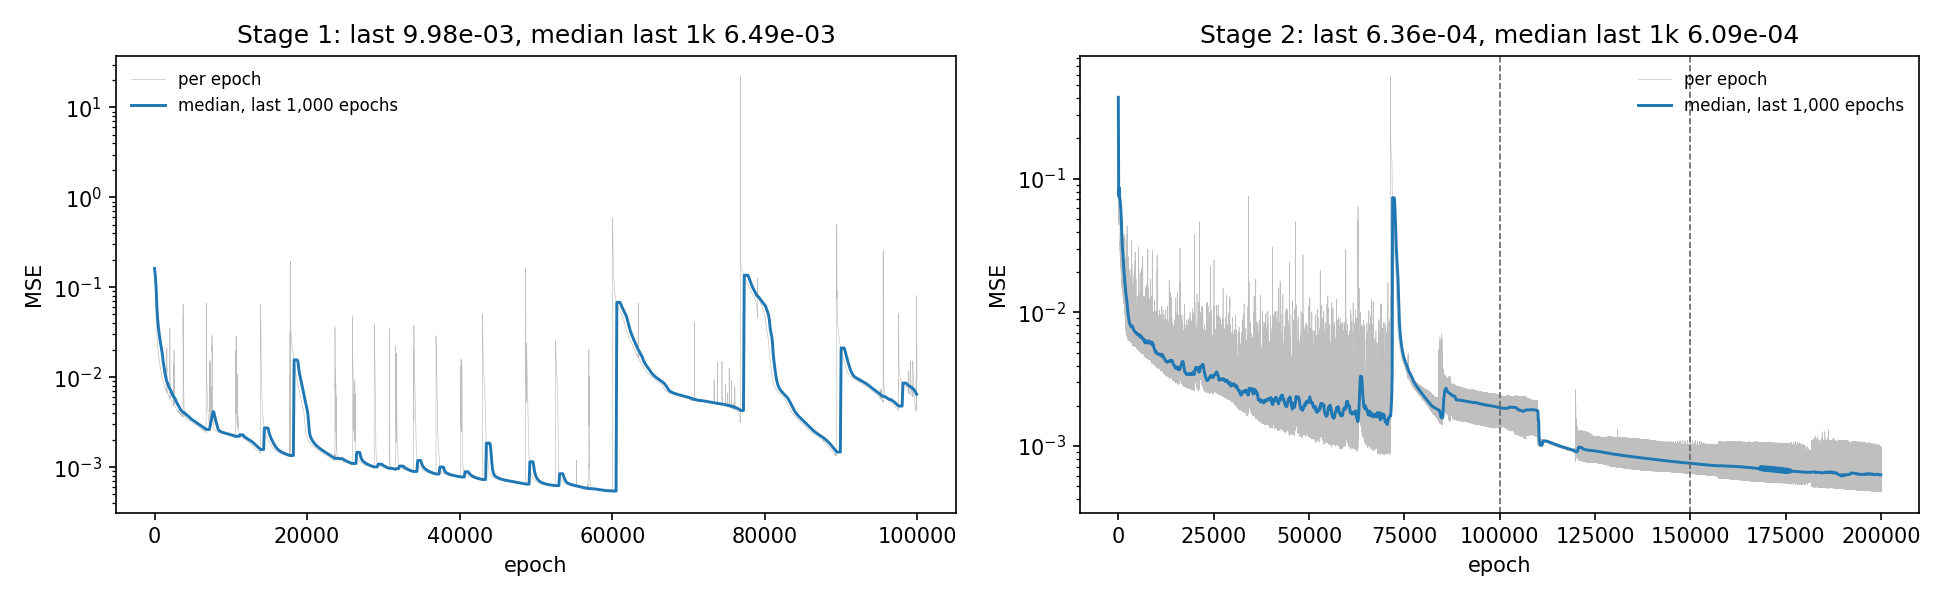
\includegraphics[
    width=0.95\textwidth,
    height=0.72\textheight,
    keepaspectratio
]{ChemKAN_report_assets/hydrogen_loss_curves_stage1_stage2_200k.png}
\caption{Hydrogen ChemKAN training histories
for Stage~1 and Stage~2. Stage~1 was trained
for 100,000 epochs, followed by 200,000
Stage-2 epochs. The stages have different
prediction targets and the loss magnitudes
should not be interpreted as directly
comparable measures of difficulty.}
\label{fig:hydrogen_training_history}
\end{figure}

\begin{figure}[H]
\centering
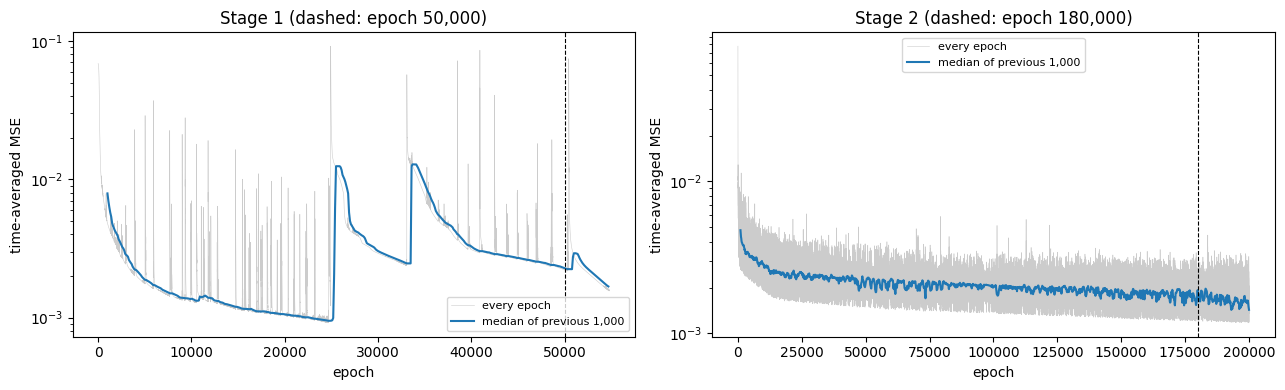
\includegraphics[width=1\textwidth]
{ChemKAN_report_assets/methane_training_histories.png}
\caption{Methane Stage-1 and Stage-2 training
histories (seed 0). Grey curves show the logged
time-averaged MSE at each epoch, while blue
curves show the median over the preceding
1,000 epochs. Dashed vertical lines indicate
the archived Stage-1 checkpoint used to initialize Stage~2 (50k) and Stage-2 evaluation checkpoint (180k).
Stage~2 training continued to 200k.
The two stages have different prediction
targets and their loss magnitudes are not
directly comparable.}
\label{fig:methane_training_history}
\end{figure}

\newpage
\section{Additional Interpretability Plots}
\label{app:interpretability}

\begin{figure}[hb]
\centering
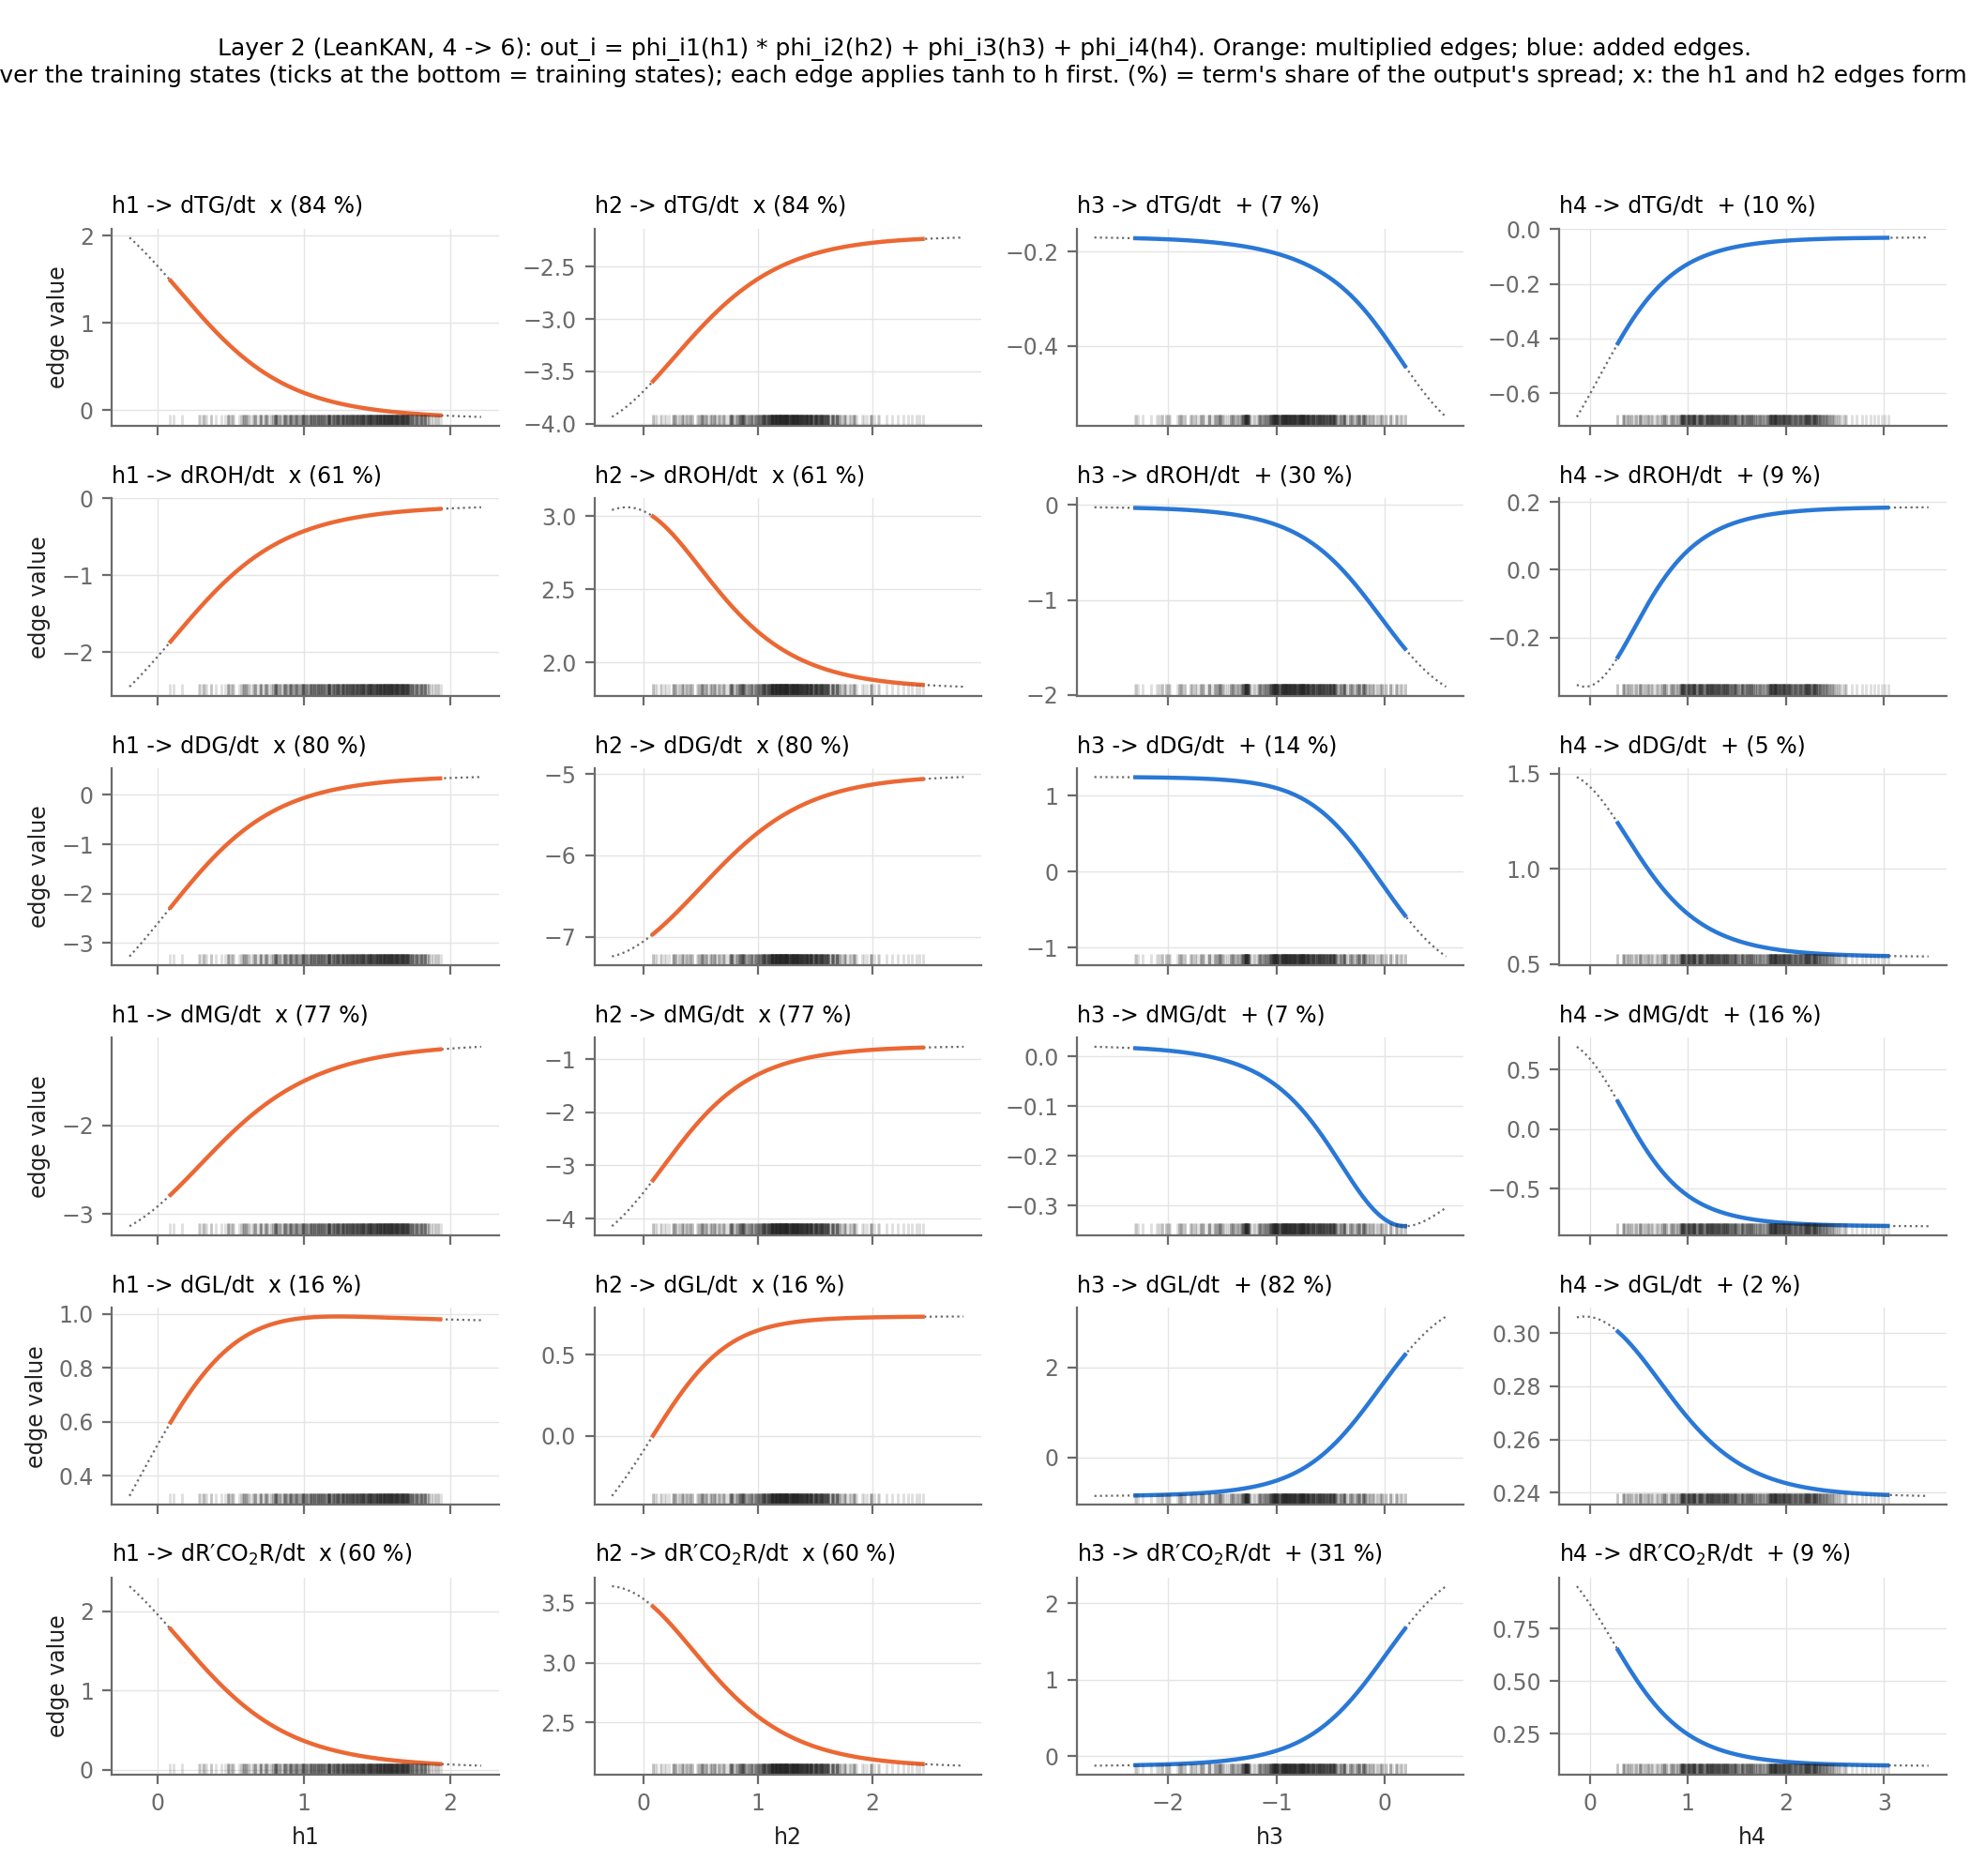
\includegraphics[
    width=1\textwidth,
    keepaspectratio
]{ChemKAN_report_assets/interpretability_biodiesel_edges_layer2.png}
\caption{Learned second-layer LeanKAN functions
in the biodiesel kinetic model. Orange curves
represent the two factors forming each
multiplicative contribution, while blue curves
represent additive contributions. The displayed
percentages indicate each output term's standard
deviation as a proportion of the sum of term
standard deviations over the training states.
Both orange factors share the percentage of
their combined product term. These values
do not imply causal feature importance.}
\label{fig:interpretability_layer2}
\end{figure}

\end{document}
